\pdfoutput=1
\documentclass[11pt]{amsart}
\usepackage{amsmath,amssymb,amsthm}
\usepackage[margin=1.2in]{geometry}
\usepackage{booktabs,adjustbox,graphicx,xcolor,placeins}
\usepackage[colorlinks=true,linkcolor=blue,citecolor=blue,urlcolor=blue]{hyperref}
\hypersetup{pdfauthor={Bernd Johannes Wuebben},
 pdftitle={Mass increase and acyclic cancellation for phase flows on quiver complexes}}
\setlength{\emergencystretch}{2em}
\newtheorem{theorem}{Theorem}[section]
\newtheorem{proposition}[theorem]{Proposition}
\newtheorem{lemma}[theorem]{Lemma}
\newtheorem{corollary}[theorem]{Corollary}
\theoremstyle{definition}
\newtheorem{definition}[theorem]{Definition}
\newtheorem{example}[theorem]{Example}
\theoremstyle{remark}
\newtheorem{remark}[theorem]{Remark}
\newcommand{\CC}{\mathbb C}
\newcommand{\RR}{\mathbb R}
\newcommand{\id}{I}
\newcommand{\HS}{\mathrm{HS}}
\newcommand{\ac}{\mathrm{ac}}
\newcommand{\ii}{\mathrm i}
\DeclareMathOperator{\tr}{tr}
\DeclareMathOperator{\Arg}{Arg}
\DeclareMathOperator{\Ein}{Ein}
\DeclareMathOperator{\Rea}{Re}
\DeclareMathOperator{\Ima}{Im}
\DeclareMathOperator{\diag}{diag}
\DeclareMathOperator{\GL}{GL}
\DeclareMathOperator{\U}{U}
\DeclareMathOperator{\polar}{polar}
\newcommand{\norm}[1]{\left\lVert#1\right\rVert}
\newcommand{\inner}[2]{\left\langle#1,#2\right\rangle}

\title[Phase flows on quiver complexes]{Mass increase and acyclic cancellation\\
for phase flows on quiver complexes}
\author{Bernd Johannes Wuebben}
\email{wuebben@gmail.com}
\subjclass[2020]{16G20, 34D05 (primary); 15A23, 53D20 (secondary)}
\keywords{Quiver representation, complex, polar decomposition, phase flow,
acyclic cancellation, K\"ahler quotient}
\date{November 2, 2026}

\begin{document}
\begin{abstract}
For two-term complexes over a two-vertex parallel-arrow quiver, with
degree-one term supported at the source, trace-norm mass can increase
along the Haiden--Katzarkov--Kontsevich--Pandit phase flow defined by
positivity. We give an explicit noncommuting example. Nevertheless, for
invertible source differential and vertex charges in the strict upper
half-plane, every positive initial metric yields exponential decay of
the acyclic coefficients and convergence of the normalized cohomology
metric. For a balanced rank-two three-arrow family, a sufficiently large
initial acyclic scale gives quantitative cancellation for arbitrary
bounded mixing, uniformly through a change of cohomology stabilizer.
The evolving coefficient approaches its instantaneous cohomology
coefficient; the proof controls the polar phase using only the
nonsingular cohomology block. As the differential scale tends to infinity,
the static mass and its first derivatives in bounded arrow coordinates
converge uniformly. A rescaled profile forces third derivatives to diverge.
An explicit primitive
has a negative Levi direction on a complex gauge orbit and identifies
the positive limiting cohomology potential.
\end{abstract}
\maketitle

\section{Introduction}\label{sec:introduction}

Haiden, Katzarkov, Kontsevich and Pandit associate a mass and a metric
phase flow to a complex of quiver representations
\cite[\S\S4.2 and 5.4]{hkkp26}. Their construction uses a coefficient
of a superconnection exponential. Acyclic summands should disappear when
the differential becomes large in the evolving metric, leaving the
cohomology representation. Question~5.18 of \cite{hkkp26} asks whether
the mass is nonincreasing along the flow. We give a negative answer for
the phase determined by their positivity condition and degree branches.
We then prove that quantitative acyclic cancellation can hold despite
this failure.

The distinction between dissipation and cancellation is essential.
The first concerns the sign of a derivative at a finite metric. The
second requires the differential to escape to infinity under the
actual equation, together with estimates on the coupled arrows.
Prescribing a large differential and computing a static limit does not
establish that a trajectory enters this regime.

\subsection{The complexes and their phase flow}
Fix a quiver with two vertices and $k$ arrows from the first vertex to
the second. We consider the two-term complex
\begin{equation}\label{eq:complex}
 (V\xrightarrow{(A_1,\ldots,A_k)}W)
 \xrightarrow{(D,0)}(U\longrightarrow0),
\end{equation}
in degrees zero and one. The chain condition is automatic. All vector
spaces are finite dimensional over $\CC$; the Hermitian metrics vary,
whereas the complex maps are fixed. The central charges $z_0,z_1$ have
strictly positive imaginary parts.

Section~\ref{sec:coefficients} derives the coefficient
$\Omega=\Omega_V\oplus\Omega_U\oplus\Omega_W$ explicitly.
On a block of degree $q$, the matrix $T=(-1)^q\Omega$ has strictly
positive imaginary part. If $T=U_T|T|$ is its polar decomposition, set
\begin{equation}\label{eq:phaseintro}
 \Phi=\Arg U_T-\pi q\id,\qquad
 m(h)=\norm{\Omega_V}_1+\norm{\Omega_U}_1+\norm{\Omega_W}_1,
 \qquad h^{-1}\dot h=-\Phi .
\end{equation}
Here $\Arg U_T$ has spectrum in $(0,\pi)$ and
$\norm{M}_1=\tr(M^\dagger M)^{1/2}$ is the trace norm.
For a single matrix, an unadorned norm denotes the operator norm.
Squared lengths of arrow tuples are sums of squared Hilbert--Schmidt
norms, denoted by the subscript $\HS$ on each arrow.
This is the unique phase in the specified branch for which
$\Omega e^{-\ii\Phi}$ is positive definite. In particular, it realizes
the positivity definition of \cite[\S4.2]{hkkp26}.

The coefficient need not be normal, contrary to the normality assertion
in \cite[Lemma~5.16]{hkkp26}. We exhibit a small example in
Section~\ref{sec:coefficients}. This issue is separate from the mass
counterexample: positivity still defines a smooth Hermitian phase, and
the metric equation exists for every finite positive time.
Throughout the paper, the phase means \eqref{eq:phaseintro}, not an
analytic logarithm of a nonnormal coefficient.

\subsection{Mass increase and cancellation}
The following two statements describe different properties of the same
equation.

\begin{theorem}\label{thm:introincrease}
Let $V=U=\CC^2$, $W=\CC$, $k=1$, and take standard initial metrics with
\[
 D=\begin{pmatrix}1/5&0\\0&2\end{pmatrix},\qquad
 A=\begin{pmatrix}1&2\end{pmatrix},\qquad
 z_0=1+\ii\epsilon,\quad z_1=4+\ii\epsilon .
\]
For every sufficiently small $\epsilon>0$, the initial derivative of
$m$ along \eqref{eq:phaseintro} is strictly positive.
\end{theorem}

The proof in Section~\ref{sec:increase} reduces the sign to a finite
real calculation with a positive interval bound. The endpoint
$\epsilon=0$ is used only as a one-sided limit; it is not an admissible
central charge. No particular positive upper endpoint for $\epsilon$
is needed for the theorem.

\begin{theorem}\label{thm:introcancellation}
Suppose that $D:V\to U$ is invertible, $\dim V=\dim U=n\geq1$ and
$\dim W=m_0\geq1$. Allow arbitrary $k$ arrows, arbitrary positive initial
metrics, and arbitrary $z_0,z_1$ in the strict upper half-plane.
Put $a=\arg z_1$. The phase flow exists for all $t\geq0$. In moving
orthonormal frames, with $X_j=A_jD^{-1}$, there are constants $C,C'>0$
depending on the initial data and charges such that
\begin{align}
 \sum_j\norm{X_j(t)}_{\HS}^2
 &\leq e^{-at}\sum_j\norm{X_j(0)}_{\HS}^2,\label{eq:introX}\\
 \lambda_{\min}(D^\dagger D)(t)&\geq at-C,\label{eq:introlambda}\\
 0\leq m(h(t))-m_0|z_1|&\leq C'e^{-at}.\label{eq:intromass}
\end{align}
The acyclic coefficient blocks tend to zero and
$\Omega_W\to z_1\id_W$ at the same exponential rate in the evolving
trace norms. In fixed coordinates on $W$, the metric
$e^{at}h_W(t)$ converges exponentially to a positive definite limit.
\end{theorem}

The proof uses the exact contraction equation for $A_jD^{-1}$.
A weighted polar estimate then forces the least singular value of $D$
to grow. Neither step assumes that the mass decreases.
No simultaneous diagonalization of $D^\dagger D$ and
$\sum_j A_j^\dagger A_j$ is imposed.

\subsection{Cancellation with arbitrary surviving cohomology}
When $\ker D$ is nonzero, the cohomology has both a source and a target.
The ratio equation acquires an additional term, which can still be
controlled without a stability or balance assumption on the surviving
representation. Let $H=\CC^{n_s}$, $W=\CC^{n_w}$, $U=\CC^r$ and
$V=H\oplus\CC^r$, with $n_s,n_w,r\geq1$. In initial adapted
orthonormal frames take arbitrary arrows $B_j:H\to W$ and set
\begin{equation}\label{eq:mixedinitial}
 D(0)=[0,F_0],\qquad A_j(0)=[B_j,T_j],\qquad
 F_0\in\GL(r,\CC),\quad \sum_j\norm{T_j}_{\HS}^2\leq M^2.
\end{equation}
Fix any charges $z_0,z_1$ in the strict upper half-plane and put
$a=\arg z_1$. Only the least singular value of $F_0$ will be constrained.
Its other singular values may be arbitrarily large.

Along the flow use the orthogonal splitting
$V=\ker D\oplus(\ker D)^\perp$ and write $D=[0,F]$, $A_j=[H_j,T_j]$.
Let $\Omega_H$ be the ordinary degree-zero coefficient of the
instantaneous surviving arrows $H_j$, and let $m_H$ be its trace-norm
mass. Its inclusion into the full graded space places zero in the
acyclic blocks. Put
\[
 q=\sum_j\norm{H_j}_{\HS}^2,\qquad
 s=\sum_j\norm{T_jF^{-1}}_{\HS}^2,\qquad
 \lambda=\sigma_{\min}(F)^2,\quad\lambda_0=\lambda(0),
\]
and set
\[
 Q=\tfrac12\bigl(m_H(0)-n_s\Rea z_0+n_w\Rea z_1\bigr)+1.
\]
The elementary mass bound in Section~\ref{sec:mixed} gives
$Q\geq q(0)+1$.

\begin{theorem}\label{thm:intromixed}
There are $\Lambda_*(Q,M,z_0,z_1)$ and
$C(n_s,n_w,r,Q,M,z_0,z_1)$ such that every initial complex
\eqref{eq:mixedinitial} with
$\sigma_{\min}(F_0)\geq\Lambda\geq\Lambda_*$ has a global phase flow
satisfying $q(t)\leq Q-3/4$ and
\begin{equation}\label{eq:intromixedratios}
 s(t)\leq M^2\Lambda^{-2}e^{-at/2},\qquad
 \lambda(t)\geq\max\{\lambda_0,at/4-C\}.
\end{equation}
Moreover,
\begin{equation}\label{eq:intromixed}
 \norm{\Omega(t)-(\Omega_H(t)\oplus0_{\ac})}_1+
 |m(h(t))-m_H(t)|\leq C\Lambda^{-2}e^{-at/8}.
\end{equation}
The constants are independent of arrow count, the surviving stabilizer
and the condition number of $F_0$. They can be chosen uniformly when
the surviving dimensions, acyclic rank, charges and total initial
arrow-norm bounds are fixed. No balance or stability hypothesis is required.
\end{theorem}

Section~\ref{sec:mixed} gives explicit constants and a threshold
independent of acyclic rank. The charges are fixed in these uniformity
statements; no uniformity as their imaginary parts vanish is asserted.
For example, acyclic singular values $\Lambda$ and $R\Lambda$ are
permitted with the same constants for every $R\geq1$.

The theorem compares with evolving cohomology. It does not assert that
cohomology itself approaches balance. The proof uses the ordinary
cohomology mass to bound $q$, and a polar estimate using only the
nonsingular cohomology block to control the additional coupling.
A separate weighted phase estimate forces growth of the acyclic
differential. These arguments make no use of full-complex mass
dissipation or of a positive orbit Hessian gap.

\subsection{Relaxation from finite cohomology energy}
Now suppose $n_s=n_w=n$ and $z_0=-1+\ii$, $z_1=1+\ii$.
Define the moment-map defects
\[
 \mu_s=\sum_jH_j^\dagger H_j-\id,\qquad
 \mu_w=\sum_jH_jH_j^\dagger-\id,\qquad
 \norm\mu^2=\norm{\mu_s}_{\HS}^2+\norm{\mu_w}_{\HS}^2.
\]
In fixed holomorphic coordinates let $h_s,h_w$ be the induced metrics
on $\ker D,W$, both multiplied by $e^{\pi t/2}$.
Using the initial orthonormal determinant volume forms, define the
cohomology Kempf--Ness function on all positive metric pairs by
\[
 \mathcal K=q+\log\det h_s-\log\det h_w.
\]

\begin{theorem}\label{thm:relaxation}
Under the hypotheses of Theorem~\ref{thm:intromixed}, with these equal
dimensions and charges, suppose
$\mathcal K_*:=\inf\mathcal K> -\infty$ and put
$E_0=\mathcal K(0)-\mathcal K_*$. Set $J_Q=1+(Q-1)^2$.
Then
\begin{equation}\label{eq:intromixedenergy}
 \begin{gathered}
 0\leq\mathcal K(t)-\mathcal K_*,\\
 \mathcal K(t)-\mathcal K_*+
 \frac1{2J_Q}\int_0^t\norm{\mu(u)}^2\,du
 \leq E_0+C_{\mathrm{en}}(Q,M)\Lambda^{-4}.
 \end{gathered}
\end{equation}
Both moment-map defects tend to zero and $m(h(t))\to2n$.
The infimum need not be attained, and initial balance is not required.
\end{theorem}

A balanced metric pair attains a finite minimum by geodesic convexity,
but its value depends on the chosen determinant normalization.
Section~\ref{sec:mixed} also gives a finite, unattained example.
A uniform energy bound across initial metrics retains a bound on $E_0$.
Neither this theorem nor the cancellation estimate asserts a uniform
final relaxation rate or convergence of normalized surviving metrics.

The initially balanced case has a particularly simple normalization.
Suppose
\begin{equation}\label{eq:initialbalance}
 \sum_jB_j^\dagger B_j=\sum_jB_jB_j^\dagger=\id_n.
\end{equation}
Then $q(0)=n$, $m_H(0)=2n$, $Q=2n+1$ and
$\mathcal K_* =\mathcal K(0)=n$.

\begin{corollary}\label{cor:balanced}
For \eqref{eq:initialbalance}, the preceding conclusions hold with
threshold $\Lambda_*(n,M)$ and constants $C(n,r,M)$, uniformly over
all balanced tuples. In particular $q(t)\leq2n+1/4$, the cancellation
rate in \eqref{eq:intromixed} is $\pi/32$, and
\eqref{eq:intromixedenergy} holds with $E_0=0$ and $J_Q=1+4n^2$.
\end{corollary}

No individual arrow is required to be invertible, and the surviving
representation need not be irreducible.

The following family makes the stabilizer uniformity explicit. Let
$n=r=2$, $k=3$, and put
\begin{equation}\label{eq:balancedfamily}
 B_1=c\id,\qquad B_2=c\sigma_z,\qquad B_3=c\epsilon\sigma_x,\qquad
 c=(2+\epsilon^2)^{-1/2},\quad 0\leq\epsilon\leq1,
\end{equation}
where
$\sigma_z=\diag(1,-1)$ and
$\sigma_x=\left(\begin{smallmatrix}0&1\\1&0\end{smallmatrix}\right)$.

\begin{corollary}\label{cor:pauli}
For \eqref{eq:balancedfamily}, $F_0=\Lambda\id_2$ and every mixing
tuple with $\sum_j\norm{T_j}_{\HS}^2\leq M^2$, the conclusions of
Corollary~\ref{cor:balanced} hold for $\Lambda\geq\Lambda_*(2,M)$,
uniformly in $\epsilon\in[0,1]$. The cohomology automorphism algebra
is scalar for $\epsilon>0$ and diagonal for $\epsilon=0$.
\end{corollary}

\begin{proof}
Both Gram sums in \eqref{eq:initialbalance} are $\id_2$.
Since $B_1=c\id$ is invertible, an automorphism is a common source
and target matrix commuting with $\sigma_z$ and $\epsilon\sigma_x$.
The first condition makes it diagonal, and the second makes it scalar
when $\epsilon>0$. The estimates follow from Corollary~\ref{cor:balanced}.
\end{proof}

The parameter $\epsilon$ is fixed along each trajectory, but may
approach zero independently of $\Lambda$ across the family.

\subsection{Static regularity and potentials}
The coefficient formulas yield an exact complex primitive in metric
directions. For an arbitrary fixed differential with least acyclic singular
value $\Lambda$, the relative primitive and its bounded-arrow-coordinate
derivatives have error $O(\Lambda^{-2})$. The mass has a $C^1$ limit with
first-derivative error $O(\Lambda^{-1})$. These bounds do not give arbitrary
derivative estimates for the polar positive factor or its phase.

On the balanced family \eqref{eq:balancedfamily}, with fixed nonzero
mixing, the mass converges in $C^2$ but its Hessian has no uniform
positive H\"older bound. A shrinking-scale profile also implies divergence
of third derivatives at points approaching $\epsilon=0$, and of the
fourth derivative at $\epsilon=0$. Thus the static cancellation limit
does not have unrestricted smooth parameter dependence.
The real phase combination of the primitive also has a negative
ambient Levi direction. Section~\ref{sec:geometry} therefore separates
the positive limiting cohomology potential from a more restricted
finite-scale positive construction. In that construction the quotient
comparison is an exact scalar isometry. It is not a metric on the
full space of arbitrary mixed complexes.

\subsection{Relation to earlier work}
In the zero-arrow case, the differential rescaling and cancellation
mechanism already appear in \cite[Example~4.1]{hkkp26}.
The motivating large-differential discussion in \cite[\S5.4]{hkkp26}
is a static comparison. Our results concern the actual coupled phase
equation and prove that its solutions enter the required regime.
The ordinary quiver metric flow studied in \cite[\S5]{hkkp20}
has a different vector field; its asymptotic results do not by themselves
apply to \eqref{eq:phaseintro}.

Superconnection localization to cohomology and heat-transgression
primitives have classical precedents. Bismut--Lott
\cite[Theorems~2.13 and 2.16]{bl95} treat cohomology localization and
transgression under a prescribed graded metric rescaling.
Paradan--Vergne \cite[\S3.2, Proposition~4 in the preprint]{pv09} give heat-decay
estimates away from the noninvertibility locus for a prescribed
superconnection rescaling. We use elementary finite-dimensional
instances of these analytic ideas. The additional estimates here
control the noncommuting polar vector field, including coupling to
a surviving representation without a positive orbit gap.
The quotient constructions in the last section use classical
quiver and K\"ahler reduction \cite{king94,sj95,sl91}; their role is
to identify precisely the geometry supplied by the explicit primitive.

Sections~\ref{sec:coefficients}--\ref{sec:polar} establish the coefficient
and polar estimates. Section~\ref{sec:invertible} proves invertible-source
cancellation, Section~\ref{sec:increase} proves mass increase, and
Section~\ref{sec:mixed} treats surviving source cohomology.
Sections~\ref{sec:static}--\ref{sec:geometry} concern static regularity
and potentials.

\section{The coefficient and the positive phase}\label{sec:coefficients}

We first compute the coefficient for \eqref{eq:complex}, allowing an
arbitrary rectangular differential $D$. Adjoint symbols always refer
to the current Hermitian metrics. Put
\begin{equation}\label{eq:BCLE}
 B=D^\dagger D,\quad L=DD^\dagger,\quad
 C=\sum_j A_j^\dagger A_j,\quad E=DCD^\dagger,
 \quad P=e^{-B},\quad Q=e^{-L}.
\end{equation}
For a nonnegative Hermitian matrix $B$, define
\begin{align}
 R(B)&=\int_0^1e^{-sB}\,ds,\label{eq:R}\\
 K_B(C)&=\int_0^1e^{-(1-s)B}Ce^{-sB}\,ds,\label{eq:K}\\
 J_L(E)&=\int_{\substack{x,z\geq0\\x+z\leq1}}
                 e^{-xL}Ee^{-zL}\,dx\,dz.\label{eq:J}
\end{align}
In particular $R(0)=1$; no inverse of $B$ is implicit in this notation.

\begin{proposition}\label{prop:coefficient}
The superconnection coefficient of \cite[\S5.4]{hkkp26} on
\eqref{eq:complex}, including its degree sign, is
\begin{equation}\label{eq:coeff}
 \begin{split}
 \Omega_V&=z_0P+K_B(C),\\
 \Omega_U&=J_L(E)-z_0Q,\\
 \Omega_W&=z_1\id_W-\sum_j A_jR(B)A_j^\dagger.
 \end{split}
\end{equation}
If $n=\dim V$, $r=\dim U$ and $m_0=\dim W$, then
\begin{equation}\label{eq:central}
 \tr\Omega=(n-r)z_0+m_0z_1.
\end{equation}
Moreover,
\begin{equation}\label{eq:imaginary}
 \Ima\Omega_V=(\Ima z_0)P,\qquad
 \Ima(-\Omega_U)=(\Ima z_0)Q,\qquad
 \Ima\Omega_W=(\Ima z_1)\id_W .
\end{equation}
\end{proposition}

\begin{proof}
We specify the graded conventions to fix the signs. In the quiver
algebra of \cite[Definition~5.13]{hkkp26}, an arrow $\alpha:s\to t$
and its adjoint have degrees $1$ and $-1$, while the vertex elements
$e_i,f_i$ have degree zero. The nontrivial two-arrow products are
$\alpha\alpha^*=\ii f_t$ and
$\alpha^*\alpha=-\ii f_s$ for a matching arrow; cross-arrow products
vanish. Products involving an $f_i$ and an arrow, and products of two
$f_i$'s, vanish. Tensor multiplication has the Koszul sign
\[
 (x\otimes T)(y\otimes S)=(-1)^{|T||y|}xy\otimes TS.
\]
The involution on an even endomorphism is the ordinary adjoint, and
on an odd endomorphism it is $\ii$ times that adjoint.
The source superconnection and curvature are
\[
 \mathsf A=\sum_i e_i\otimes d_i+\sum_j\alpha_j\otimes A_j,\qquad
 F=(\mathsf A-\mathsf A^*)^2+\ii\sum_i f_i\otimes z_i.
\]
The coefficient is
$\Omega=(-1)^{\deg}\exp(-\ii F)_f$, where the subscript means
coefficient extraction after exponentiation.

Write $X=-\ii F$. Its vertex part is $-B$ on $V$, $-L$ on $U$
and zero on $W$. Its $f$ coefficients before exponentiation are
$C+z_0\id$ on $V$, $z_0\id$ on $U$, and
$z_1\id-\sum_j A_jA_j^\dagger$ on $W$.
Its mixed arrow terms are $-A_jD^\dagger:U\to W$ and
$-\ii DA_j^\dagger:W\to U$, with their respective algebra factors.
Their paired $f$ contribution is $-DCD^\dagger$ on $U$ and
$\sum_j A_jD^\dagger DA_j^\dagger$ on $W$.

The Duhamel expansion contributing to an $f$ coefficient terminates
at one $f$ insertion or two arrow insertions. There are no mixed
paths on $V$, giving $K_B(C)+z_0P$. On $U$, the two-insertion term
is $-J_L(E)$ before multiplication by the degree-one sign.
On $W$ the two-insertion contribution is
\[
 \sum_j\int_0^1(1-s)A_jD^\dagger e^{-sL}DA_j^\dagger\,ds.
\]
Using $D^\dagger e^{-sL}D=Be^{-sB}$ and
\[
 -\id+\int_0^1(1-s)Be^{-sB}\,ds=-R(B)
\]
proves \eqref{eq:coeff}.

The substitutions $s\mapsto1-s$ and $(x,z)\mapsto(z,x)$ show that
$K_B(C)$ and $J_L(E)$ are Hermitian. This proves
\eqref{eq:imaginary}; neither integral operator is asserted to preserve
positivity. Cyclicity of trace gives
\[
 \tr K_B(C)=\tr(CP),\qquad
 \tr J_L(E)
 =\tr\left(C\int_0^1sBe^{-sB}\,ds\right)
 =\tr(C(R(B)-P)).
\]
The arrow traces cancel. The nonzero spectra of $B$ and $L$ agree,
so $\tr P-\tr Q=n-r$, proving \eqref{eq:central}.
\end{proof}

\begin{lemma}\label{lem:phase}
If $\Ima T>0$ and $T=U_T|T|$ is its polar decomposition, then
every eigenvalue of $U_T$ lies in the open upper semicircle.
On a block of degree $q$, the matrix
$\Phi=\Arg U_T-\pi q\id$ is the unique Hermitian matrix with spectrum
in $(-\pi q,\pi(1-q))$ such that
$(-1)^qT e^{-\ii\Phi}$ is positive definite.
\end{lemma}

\begin{proof}
For a unit eigenvector $v$ of $U_T$ with eigenvalue $e^{\ii\theta}$,
\[
 0<\inner{v}{\Ima(T)v}
   =\sin\theta\,\inner{v}{|T|v}.
\]
Thus $0<\theta<\pi$. With the stated branch,
$(-1)^qT e^{-\ii\Phi}=TU_T^\dagger=(TT^\dagger)^{1/2}>0$.
Conversely positivity identifies $e^{\ii\Phi}$ as the polar unitary
of $(-1)^qT$. Uniqueness of polar decomposition and of the branch
give uniqueness of $\Phi$.
\end{proof}

For the trace functional $\mathcal L(a)=\tr(\Omega a)$,
the positivity requirement
$\mathcal L(e^{-\ii\Phi}a^\dagger a)\geq0$ for all $a$
is exactly the positivity of $\Omega e^{-\ii\Phi}$.
Lemma~\ref{lem:phase} therefore identifies the phase required by
\cite[\S4.2]{hkkp26} without a normality hypothesis.
The degree convention also respects shifts: the shift $[1]$ moves
degree $q$ to $q-1$ and increases the phase by $\pi$.
Orthogonal direct sums give direct sums of coefficients and phases,
and additive mass.

\begin{example}\label{ex:nonnormal}
Take $V=U=W=\CC^2$, $z_0=z_1=\ii$,
$D=\diag(1,\sqrt2)$ and
$A=\left(\begin{smallmatrix}1&1\\0&1\end{smallmatrix}\right)$.
Writing $p=e^{-1}$ and $q=e^{-2}$, formula \eqref{eq:coeff} gives
\[
 \Omega_V=
 \begin{pmatrix}(1+\ii)p&p-q\\p-q&(2+\ii)q\end{pmatrix},\qquad
 [\Omega_V,\Omega_V^\dagger]
 =2\ii(p-q)^2\begin{pmatrix}0&1\\-1&0\end{pmatrix}\ne0.
\]
Thus coefficient extraction does not preserve the normality of an
element in the graded algebra. This example contradicts the
normality clause of \cite[Lemma~5.16]{hkkp26}, while retaining the
strict imaginary-part property and the central-charge trace.
\end{example}

\subsection{Variation and global existence}
At an instant choose orthonormal frames. Along the metric phase flow,
the fixed maps have moving-frame derivatives
\begin{equation}\label{eq:mapflow}
 \dot D=\tfrac12(D\Phi_V-\Phi_UD),\qquad
 \dot A_j=\tfrac12(A_j\Phi_V-\Phi_WA_j).
\end{equation}
For example, a variation $\xi_q=h_q^{-1}\delta h_q$ gives
$\delta D=(\xi_UD-D\xi_V)/2$ and
$\delta A_j=(\xi_WA_j-A_j\xi_V)/2$ in such frames.
Substituting $\xi=-\Phi$ gives \eqref{eq:mapflow}.

All coefficient variations can be computed without denominators involving
eigenvalue differences. Define block matrices
\[
 N_V=\begin{pmatrix}-B&C\\0&-B\end{pmatrix},\quad
 N_U=\begin{pmatrix}-L&E&0\\0&0&\id\\0&0&-L\end{pmatrix},\quad
 N_R=\begin{pmatrix}-B&\id\\0&0\end{pmatrix}.
\]
Then $(e^{N_V})_{11}=P$, $(e^{N_V})_{12}=K_B(C)$,
$(e^{N_U})_{11}=Q$, $(e^{N_U})_{13}=J_L(E)$ and
$(e^{N_R})_{12}=R(B)$. The Fr\'echet derivative
\begin{equation}\label{eq:duhamel}
 \mathrm D\exp_N(\dot N)=\int_0^1e^{(1-s)N}\dot N e^{sN}\,ds
\end{equation}
and the product rule therefore determine every $\dot\Omega_q$.
In particular,
\[
 \dot\Omega_W=-\sum_j\bigl(\dot A_jRA_j^\dagger+
 A_j\dot R A_j^\dagger+A_jR\dot A_j^\dagger\bigr).
\]

\begin{lemma}\label{lem:massvariation}
Let $\Omega_q=U_q|\Omega_q|$ on each homogeneous block. Then
\begin{equation}\label{eq:massvariation}
 \dot m=\sum_q\Rea\tr(U_q^\dagger\dot\Omega_q).
\end{equation}
The coefficients and phase define a smooth metric vector field, whose
solutions exist for all $t\geq0$.
\end{lemma}

\begin{proof}
For an invertible matrix $\Omega=UH$, differentiation of
$H^2=\Omega^\dagger\Omega$ and taking trace after multiplication by
$H^{-1}$ gives
$\tr\dot H=\Rea\tr(U^\dagger\dot\Omega)$.
This proves \eqref{eq:massvariation}.
The polar decomposition and its upper-semicircle logarithm are smooth
on the domain in Lemma~\ref{lem:phase}.
If a phase derivative is needed, put
$S=U^\dagger\dot U$ and $Z=U^\dagger\dot\Omega$; it is determined by
\[
 HS+SH=Z-Z^\dagger,\qquad S^\dagger=-S,
\]
followed by differentiation of the chosen unitary logarithm.
The Sylvester operator is invertible because $H>0$.

The branches give $0<\Phi_V,\Phi_W<\pi\id$ and
$-\pi\id<\Phi_U<0$. In fixed coordinates the metric forms satisfy
\[
 e^{-\pi t}h_V(0)\leq h_V(t)\leq h_V(0),\qquad
 h_U(0)\leq h_U(t)\leq e^{\pi t}h_U(0),
\]
and the same degree-zero bounds hold on $W$.
On every finite time interval these inequalities confine the metrics
to a compact subset of the positive cone. The smooth ordinary
differential equation therefore extends past every finite time.
\end{proof}

\section{Polar estimates uniform under degeneration of a complementary block}\label{sec:polar}

A bound for the full polar factor based on the least singular values,
such as \cite{li95}, can deteriorate when a singular value approaches zero.
Polar approximation and trace-norm variational principles are classical
\cite{higham86,lewis95}. The acyclic coefficient has
exponentially small singular values, so such a bound would be unsuitable
here. The following estimates use only the surviving block or one
specified reference direction. All Hilbert--Schmidt norms in this
section are for fixed orthonormal frames.

\begin{lemma}\label{lem:partialpolar}
Let
\[
 T=\begin{pmatrix}A&E\\E^\dagger&C\end{pmatrix},\qquad \Ima T>0,
\]
and suppose that the least singular value of $A$ is at least $b>0$.
Let $U=\polar(T)$, $U_A=\polar(A)$ and $e=\norm{E}_{\HS}$.
Then
\begin{equation}\label{eq:polarblocks}
 \norm{U_{12}}_{\HS}=\norm{U_{21}}_{\HS}\leq4e/b,\qquad
 \norm{U_{11}-U_A}_{\HS}\leq2e/b.
\end{equation}
Writing $\Psi=\Arg U$ and $\psi_A=\Arg U_A$, one has
\begin{equation}\label{eq:phaseoff}
 \norm{\Psi_{12}}_{\HS}\leq2\pi e/b.
\end{equation}
If $e/b\leq1/8$, then also
\begin{equation}\label{eq:phasecompressed}
 \norm{\Psi_{11}-\psi_A}_{\HS}\leq4\pi e/b .
\end{equation}
There is no lower bound on the singular values of $C$ or $T$ in these
estimates.
\end{lemma}

\begin{proof}
Put $v=\norm{U_{12}}_{\HS}=\norm{U_{21}}_{\HS}$, where equality follows
by taking traces in the unitary row and column identities.
Pinching is contractive for the trace norm, so
$\norm{T}_1\geq\norm{A}_1+\norm{C}_1$.
In the maximizing pairing $\norm{T}_1=\Rea\tr(U^\dagger T)$,
the $C$ contribution is at most $\norm{C}_1$ because $U_{22}$ is
a contraction, and the two off-diagonal contributions have sum at most
$2ve$.
If $A=U_A|A|$ and $d=\norm{U_{11}-U_A}_{\HS}$, the deficit in
the $A$ contribution is
\[
 \tr\bigl(|A|[\id-\Rea(U_{11}^\dagger U_A)]\bigr)
 \geq \frac b2(d^2+v^2).
\]
The bracket is positive semidefinite, and its trace is
$(d^2+v^2)/2$ by the first-column unitary identity.
It follows that $d^2+(v-2e/b)^2\leq(2e/b)^2$, proving
\eqref{eq:polarblocks}.

For $\alpha,\beta\in[0,\pi]$,
\begin{equation}\label{eq:chord}
 |\alpha-\beta|\leq\frac\pi2|e^{\ii\alpha}-e^{\ii\beta}|.
\end{equation}
Expanding the commutators of $U$ and $\Arg U$ with the first-block
orthogonal projection in an eigenbasis of $U$ proves
$\norm{\Psi_{12}}_{\HS}\leq(\pi/2)v$, hence \eqref{eq:phaseoff}.
The same scalar inequality, expanded in eigenbases of two normal
matrices, gives the Hilbert--Schmidt estimate
\begin{equation}\label{eq:logHS}
 \norm{\Arg U-\Arg U_0}_{\HS}
 \leq\frac\pi2\norm{U-U_0}_{\HS}
\end{equation}
whenever both unitary spectra lie in the closed upper semicircle.

By Lemma~\ref{lem:phase}, $\Ima U>0$; its compression $U_{22}$
is invertible and its polar unitary $V$ also has upper-semicircle
spectrum. Since
$U_{22}^\dagger U_{22}=\id-U_{12}^\dagger U_{12}$,
\[
 \norm{U_{22}-V}_{\HS}
 =\norm{(\id-U_{12}^\dagger U_{12})^{1/2}-\id}_{\HS}
 \leq\norm{U_{12}^\dagger U_{12}}_{\HS}\leq v^2 .
\]
Take $U_0=\diag(U_A,V)$. If $e/b\leq1/8$, then $v\leq1/2$ and
\[
 \norm{U-U_0}_{\HS}^2=d^2+2v^2+\norm{U_{22}-V}_{\HS}^2
 \leq40(e/b)^2<64(e/b)^2.
\]
Equation~\eqref{eq:logHS} proves \eqref{eq:phasecompressed}.
\end{proof}

\begin{lemma}\label{lem:weightedpolar}
Let $T_0=U_0H_0$ be an invertible reference matrix in polar form,
and suppose that $T=T_0+E$ has $\Ima T>0$ with polar unitary $U$.
If $v$ is a unit vector satisfying
$H_0v=pv$ and $U_0v=e^{\ii\theta}v$, where $p>0$ and $0<\theta<\pi$,
then
\begin{equation}\label{eq:weightedphase}
 \left|\inner{v}{(\Arg U-\theta\id)v}\right|
 \leq\pi\sqrt{\frac{\norm{E}_1}{p}} .
\end{equation}
\end{lemma}

\begin{proof}
The trace-norm variational principle and triangle inequality imply
\[
 \tr\bigl(H_0[\id-\Rea(U^\dagger U_0)]\bigr)\leq2\norm{E}_1.
\]
The bracket is positive semidefinite, and
$H_0-pvv^\dagger\geq0$. Its expectation on $v$ is
$1-\Rea(e^{-\ii\theta}\inner{v}{Uv})$.
Writing $\Psi=\Arg U$ and using
$1-\cos x\geq2x^2/\pi^2$ for $|x|\leq\pi$ therefore gives
\[
 \frac{2p}{\pi^2}\inner{v}{(\Psi-\theta\id)^2v}
 \leq2\norm{E}_1.
\]
Cauchy--Schwarz proves the assertion.
\end{proof}

The frequently used special case is $T=zP+E$, $P>0$, $\Ima z>0$.
For an eigenvector $Pv=p_0v$, \eqref{eq:weightedphase} becomes
\begin{equation}\label{eq:weightedscalar}
 \left|\inner{v}{(\Arg\polar(T)-\arg z)v}\right|
 \leq\pi\sqrt{\frac{\norm{E}_1}{|z|p_0}}.
\end{equation}
The estimate is useful even when no uniform lower bound for all
eigenvalues of $P$ is available. Later it is applied to a direction
realizing the least singular value of the differential, for which
$p_0$ is known exactly.

\section{Cancellation for an invertible differential}\label{sec:invertible}

We prove Theorem~\ref{thm:introcancellation}. The surviving cohomology
is $W$ in degree zero. Put $a=\arg z_1\in(0,\pi)$ and, in moving
orthonormal frames, define
\begin{equation}\label{eq:invertiblevariables}
 X_j=A_jD^{-1},\qquad H_X=\sum_jX_j^\dagger X_j,\qquad
 s=\tr H_X,\qquad \lambda=\lambda_{\min}(D^\dagger D).
\end{equation}

\begin{lemma}\label{lem:Xcontract}
Along the phase flow,
\begin{equation}\label{eq:Xcontract}
 \dot X_j=\tfrac12(X_j\Phi_U-\Phi_WX_j),\qquad
 s(t)\leq s(0)e^{-at}.
\end{equation}
\end{lemma}

\begin{proof}
Differentiate $A_jD^{-1}$ using \eqref{eq:mapflow}; the source phase
cancels. Since $A_j=X_jD$,
\begin{equation}\label{eq:targetX}
 \Omega_W=z_1\id-\sum_jX_j(\id-e^{-L})X_j^\dagger .
\end{equation}
The subtracted matrix is positive semidefinite. This target block
is normal, with scalar strictly positive imaginary part, and
$\arg(z_1-r)\geq\arg z_1$ for $r\geq0$. Thus $\Phi_W\geq a\id$,
whereas $\Phi_U<0$ on the degree-one branch. Consequently
\[
 \dot s=\sum_j\tr(X_j^\dagger X_j\Phi_U)
          -\tr\left(\sum_jX_jX_j^\dagger\Phi_W\right)
 \leq-as.
\]
\end{proof}

\begin{lemma}\label{lem:heatbounds}
Let $\kappa=\pi/(2e)$. For an invertible differential of rank $n$,
the coefficient terms in \eqref{eq:coeff} satisfy
\begin{equation}\label{eq:heatbounds}
 \norm{K_B(C)}_1\leq n\kappa s,\qquad
 \norm{J_L(E)}_1\leq ns,\qquad
 \norm{\Omega_W-z_1\id}_1\leq s.
\end{equation}
The constants do not depend on any singular-value ratio of $D$.
\end{lemma}

\begin{proof}
Write $D=U_DB^{1/2}$ and $S=U_D^\dagger H_XU_D$. Then
$C=B^{1/2}SB^{1/2}$, $S\geq0$ and $\tr S=s$.
For $u>0$,
$\norm{B^{1/2}e^{-uB}}\leq(2eu)^{-1/2}$.
Integration in \eqref{eq:K}, using
$\int_0^1[s(1-s)]^{-1/2}ds=\pi$, gives
$\norm{K_B(C)}\leq\kappa s$, hence the first trace-norm bound.

On $U$, $E=LH_XL$. In an eigenbasis of $L$ with eigenvalues $l_i$,
\[
 (J_L(E))_{ij}=k_{ij}(H_X)_{ij},\qquad
 k_{ij}=l_il_j\int_{\substack{x,z\geq0\\x+z\leq1}}
                  e^{-xl_i-zl_j}\,dx\,dz .
\]
Enlarging the integration region to the nonnegative quadrant gives
$0\leq k_{ij}\leq1$. Positivity of $H_X$ implies
$|(H_X)_{ij}|\leq\sqrt{(H_X)_{ii}(H_X)_{jj}}$. Therefore
\[
 |\inner{v}{J_L(E)v}|
 \leq\left(\sum_i|v_i|\sqrt{(H_X)_{ii}}\right)^2
 \leq s\norm v^2.
\]
Since $J_L(E)$ is Hermitian, this proves the second estimate.
Finally the positive semidefinite matrix subtracted in
\eqref{eq:targetX} has trace at most $s$.
\end{proof}

\begin{lemma}\label{lem:growinggap}
There is a constant $C$ depending on the initial data and charges such
that $\lambda(t)\geq at-C$ for every $t\geq0$.
\end{lemma}

\begin{proof}
The least eigenvalue $\lambda$ is locally Lipschitz. At almost every
time, choose a unit minimum eigenvector $v$ realizing its derivative,
and set $u=Dv/\sqrt\lambda$. Then $Lu=\lambda u$ and
\begin{equation}\label{eq:lambdaderivative}
 \dot\lambda
 =\lambda\bigl(\inner{v}{\Phi_Vv}-\inner{u}{\Phi_Uu}\bigr)>0.
\end{equation}
The same lower estimates hold on every vector in a repeated minimum
eigenspace, and hence for the corresponding one-sided eigenvalue
derivatives. In particular $\lambda\geq\lambda_0:=\lambda(0)>0$.

Apply \eqref{eq:weightedscalar} to
$\Omega_V=z_0e^{-B}+K_B(C)$ and
$-\Omega_U=z_0e^{-L}-J_L(E)$.
On $v$ and $u$ the reference heat eigenvalue is $e^{-\lambda}$.
The reference phases differ by $\pi$ after the degree-one branch
shift. Lemmas~\ref{lem:Xcontract} and \ref{lem:heatbounds} yield
\begin{equation}\label{eq:gapineq}
 \dot\lambda\geq\lambda
   \left[\pi-C_0e^{(\lambda-at)/2}\right],\qquad
 C_0=\pi\sqrt{\frac{ns(0)}{|z_0|}}(\sqrt\kappa+1).
\end{equation}
Let $L_0=\max\{0,2\log(2C_0/\pi)\}$, taking $L_0=0$ when $C_0=0$.
Whenever $\lambda\leq at-L_0$, the bracket in \eqref{eq:gapineq}
is at least $\pi/2$.

For completeness, choose
\[
 M_0=\max\{\lambda_0,4a/\pi,1\},\quad
 T_0=(M_0+L_0)/a,\quad
 T_1=T_0+\frac2\pi\log(M_0/\lambda_0).
\]
For $t\geq T_0$ while $\lambda\leq M_0$,
$\dot\lambda\geq\pi\lambda/2$, so $\lambda$ reaches $M_0$ by $T_1$.
The line $b(t)=M_0+a(t-T_1)$ satisfies
$b(t)-at=M_0-aT_1\leq-L_0$.
At a contact point $\lambda=b$ for $t\geq T_1$,
$\dot\lambda\geq\pi b/2\geq2a>\dot b$.
Scalar comparison gives $\lambda\geq b$ thereafter. Before $T_1$
we have $\lambda>0$, so $\lambda(t)\geq at-aT_1$ for all $t\geq0$.
\end{proof}

\begin{proof}[Proof of Theorem~\ref{thm:introcancellation}]
Global existence is Lemma~\ref{lem:massvariation}.
The contraction and gap statements follow from
Lemmas~\ref{lem:Xcontract} and \ref{lem:growinggap}.
The latter also gives
$\norm{e^{-B}}=\norm{e^{-L}}\leq e^{aT_1}e^{-at}$.
Thus
\begin{align*}
 \norm{\Omega_V}_1+\norm{\Omega_U}_1
 &\leq\bigl(2n|z_0|e^{aT_1}+n(\kappa+1)s(0)\bigr)e^{-at},\\
 \norm{\Omega_W-z_1\id}_1&\leq s(0)e^{-at}.
\end{align*}
The central-charge identity is $\tr\Omega=m_0z_1$.
The triangle inequality gives the lower mass bound
$m(h(t))\geq m_0|z_1|$ and, with the last two estimates, the upper
bound \eqref{eq:intromass}.

It remains to identify convergence of a metric in fixed coordinates.
For $r\geq0$,
\[
 0\leq\arg(z_1-r)-a
 =\int_0^r\frac{\Ima z_1}{|z_1-u|^2}\,du
 \leq\frac r{\Ima z_1}.
\]
Spectral calculus in \eqref{eq:targetX} yields
$0\leq\Phi_W-a\id\leq s(0)e^{-at}(\Ima z_1)^{-1}\id$.
For $\widehat h_W=e^{at}h_W$, comparison of Hermitian forms gives
\[
 e^{-s(0)/(a\Ima z_1)}h_W(0)
 \leq\widehat h_W(t)\leq h_W(0).
\]
The normalized metric is decreasing, and hence has a positive definite
limit. Its derivative in any fixed coordinate norm is $O(e^{-at})$,
by the same comparison and the phase bound. Integration proves
exponential convergence.
\end{proof}

\begin{remark}\label{rem:zero}
Zero-dimensional cases have direct descriptions. If $V=U=0$, the only
coefficient is $z_1\id_W$ and $h_W(t)=e^{-at}h_W(0)$.
If $W=0$, all arrows vanish; writing $\theta_0=\arg z_0$ gives
$\Phi_V=\theta_0\id$ and $\Phi_U=(\theta_0-\pi)\id$.
Consequently $D(t)=e^{\pi t/2}D(0)$ in moving frames and
$m(h(t))=2|z_0|\tr e^{-e^{\pi t}D(0)^\dagger D(0)}$.
Thus the acyclic mass decays faster than every fixed exponential.
\end{remark}

\section{A mass-increasing trajectory}\label{sec:increase}

We prove Theorem~\ref{thm:introincrease} by computing a positive one-sided
limit of the exact mass derivative. All metric and phase conventions
remain those of Section~\ref{sec:coefficients}.
For the initial matrices in that theorem,
$D^\dagger D=\diag(1/25,4)$ and
$A^\dagger A=\left(\begin{smallmatrix}1&2\\2&4\end{smallmatrix}\right)$
do not commute.

\subsection{The real limiting coefficient}
Put
\[
 b_1=1/25,\quad b_2=4,\quad p=e^{-b_1},\quad q=e^{-b_2},
 \quad R_i=\frac{1-e^{-b_i}}{b_i},\quad f_i=R_i-e^{-b_i},
\]
and define
\[
 \ell=\frac{p-q}{b_2-b_1},\qquad
 s_*=\frac{\sqrt{b_1b_2}(R_1-R_2)}{b_2-b_1}.
\]
At $\epsilon=0$ the coefficient blocks have the real symmetric limits
\begin{equation}\label{eq:realblocks}
 H=\begin{pmatrix}2p&2\ell\\2\ell&5q\end{pmatrix},\quad
 G=\begin{pmatrix}f_1-p&2s_*\\2s_*&4f_2-q\end{pmatrix},\quad
 w=4-R_1-4R_2=25p+q-22.
\end{equation}
The elementary bounds below give
\begin{equation}\label{eq:realblocksigns}
 \begin{gathered}
 -0.05060<\det H<-0.05059,\qquad
 -0.85991<\det G<-0.85990,\\
 2.03805<w<2.03806 .
 \end{gathered}
\end{equation}
Thus $H$ and $G$ each have one negative and one positive eigenvalue.
For a real symmetric $2$ by $2$ matrix $M$ with this property,
\begin{equation}\label{eq:negativeprojection}
 P_-(M)=\frac12\left(\id-
 \frac{2M-(\tr M)\id}{\sqrt{(\tr M)^2-4\det M}}\right).
\end{equation}
Write $P_V=P_-(H)$ and $P_U=P_-(G)$.

All limiting blocks are invertible. The polar unitary is continuous
near them. On the degree-zero branch its eigenvalues approach $1$
and $-1$ through the upper semicircle; the corresponding phases approach
$0$ and $\pi$. On the degree-one block apply the same observation to
$-\Omega_U$ and subtract $\pi$. It follows that
\begin{equation}\label{eq:phaselimit}
 \Phi_V\longrightarrow\pi P_V,\qquad
 \Phi_U\longrightarrow-\pi P_U,\qquad
 \Phi_W\longrightarrow0
 \quad(\epsilon\downarrow0).
\end{equation}
The argument is continuous on the closed upper semicircle with these
endpoint values. This assertion does not use continuity across a branch
cut from the lower semicircle.

\subsection{A finite real formula for the derivative}
Divide the limiting map velocities by $\pi$ and denote this directional
derivative by a prime. Equation~\eqref{eq:mapflow} becomes
\begin{equation}\label{eq:realvelocity}
 D'=\tfrac12(DP_V+P_UD),\qquad A'=\tfrac12AP_V .
\end{equation}
Since the central-charge trace is constant, the trace-norm derivative
formula gives
\begin{equation}\label{eq:positivelimit}
 \lim_{\epsilon\downarrow0}\frac{\dot m_\epsilon(0)}{\pi}
 =-2\tr(P_VH'+P_UG').
\end{equation}
Indeed, at the real invertible blocks the polar unitaries are their
sign matrices $\id-2P_V$, $\id-2P_U$, and $1$.
The identity contributions sum to the derivative of \eqref{eq:central},
which vanishes.

Here is a scalar-arithmetic evaluation of the right side of
\eqref{eq:positivelimit}. It avoids differentiating eigenvectors of
the coefficient. Let $B=\diag(b_1,b_2)$ and
$C=\left(\begin{smallmatrix}1&2\\2&4\end{smallmatrix}\right)$.
Set
\begin{equation}\label{eq:Bprime}
 B'=\tfrac12(P_VB+BP_V)+DP_UD,\quad
 \gamma=\frac{B'_{12}}{b_2-b_1},\quad
 K=\begin{pmatrix}0&\gamma\\-\gamma&0\end{pmatrix}.
\end{equation}
Use instantaneous singular-vector frames for $D$.
In the source frame, $B'+[B,K]$ is diagonal and
$b_i'=B'_{ii}$. The arrow Gram derivative is
\begin{equation}\label{eq:Cprime}
 \widetilde C'=\tfrac12(P_VC+CP_V)+[C,K].
\end{equation}
The corresponding target frame makes $D$ diagonal to first order.
Frame rotations do not change the traces
$\tr(P_VH')$ and $\tr(P_UG')$, since the projections commute with
the respective limiting blocks.

The remaining derivatives are
\begin{align}
 R_i'&=-\frac{f_i}{b_i}b_i',\qquad
 f_i'=\left(-\frac{f_i}{b_i}+e^{-b_i}\right)b_i',\label{eq:Rprime}\\
 \ell'&=\frac{(-pb_1'+qb_2')(b_2-b_1)
                    -(p-q)(b_2'-b_1')}{(b_2-b_1)^2},\label{eq:ellprime}\\
 s_*'&=\frac{s_*}{2}\left(\frac{b_1'}{b_1}+\frac{b_2'}{b_2}\right)\notag\\
 &\quad+\sqrt{b_1b_2}\,
  \frac{(R_1'-R_2')(b_2-b_1)-(R_1-R_2)(b_2'-b_1')}
       {(b_2-b_1)^2}.\label{eq:sprime}
\end{align}
In these frames,
\begin{align}
 H'_{ii}&=e^{-b_i}\bigl(\widetilde C'_{ii}-(1+C_{ii})b_i'\bigr),
 &H'_{12}&=\ell\widetilde C'_{12}+C_{12}\ell',\label{eq:Hprime}\\
 G'_{ii}&=f_i\widetilde C'_{ii}
 +\left[C_{ii}\left(-f_i/b_i+e^{-b_i}\right)+e^{-b_i}\right]b_i',
 &&\label{eq:Gprime}\\
 G'_{12}&=s_*\widetilde C'_{12}+C_{12}s_*'.&&\notag
\end{align}
Equations \eqref{eq:realblocks}--\eqref{eq:Gprime} are a finite expression
using rational operations, two exponentials and positive square roots.

\subsection{Strict positivity}
The two exponentials lie in the rational intervals
\begin{equation}\label{eq:expintervals}
 \begin{split}
 0.96078943915232320&<p<0.96078943915232322,\\
 0.01831563888873417&<q<0.01831563888873419.
 \end{split}
\end{equation}
To verify them, use the Taylor sums of degrees $31$ and $30$ for
$e^{-1/25}$, and of degrees $81$ and $80$ for $e^{-4}$.
The odd and even sums bound the exponential from below and above,
respectively, by the sign of the Taylor remainder. Each comparison with
the displayed decimal endpoint is a rational comparison.

Substitution in the finite formulas above, with interval operations,
gives the enclosures in Table~\ref{tab:intervals}. Each printed matrix
entry differs from its exact value by less than $10^{-8}$.
These deliberately coarse enclosures suffice to give
\begin{equation}\label{eq:coarsepositive}
 0.2395<-2\tr(P_VH'+P_UG')<0.2397.
\end{equation}
One may verify the table using only rational endpoints: every positive
square root can be enclosed by rational lower and upper bounds whose
squares enclose its argument. Thus the sign calculation does not
depend on a floating-point eigensolver or a finite-difference derivative.\footnote{The
source distribution includes two independent interval computations:
\path{figures/code/compute05_interval.py} and
\path{figures/code/compute05_independent.py}. The latter uses only
integer interval arithmetic from the Python standard library. They
enclose the one-sided limiting derivative, not a specified positive
value of $\epsilon$.}

\begin{table}[ht]
\caption{Enclosures for the sign calculation. For each symmetric matrix,
the entries are listed in the order $(11,12,22)$; each entry has error
less than $10^{-8}$.}\label{tab:intervals}
\centering
\begin{adjustbox}{max width=\textwidth,center}
\begin{tabular}{lrrr}
\toprule
Matrix & $11$ & $12$ & $22$\\
\midrule
$H$   & $1.92157888$ & $0.47599687$ & $0.09157819$\\
$G$   & $-0.94131486$ & $0.14845312$ & $0.89010617$\\
$P_V$ & $0.05643063$ & $-0.23075142$ & $0.94356937$\\
$P_U$ & $0.99355619$ & $-0.08001432$ & $0.00644381$\\
$H'$  & $0.01353176$ & $-0.24643619$ & $-0.29654199$\\
$G'$  & $0.06216737$ & $0.10644365$ & $0.12306918$\\
\bottomrule
\end{tabular}
\end{adjustbox}
\end{table}

\begin{proof}[Proof of Theorem~\ref{thm:introincrease}]
The coefficients, their directional derivatives, and the polar
unitaries extend continuously to the invertible real limiting blocks.
Equation~\eqref{eq:phaselimit} gives convergence of the actual flow
directions from $\epsilon>0$. The trace-norm derivative is consequently
continuous in this one-sided limit. Equations~\eqref{eq:positivelimit}
and \eqref{eq:coarsepositive} show that the limit is positive.
It follows that $\dot m_\epsilon(0)>0$ for all sufficiently small
$\epsilon>0$, when both central charges are admissible.
\end{proof}

The example disproves universal mass dissipation for the specified
positive phase, rather than merely exposing a failure of normality.
It does not preclude eventual cancellation, which
Theorem~\ref{thm:introcancellation} proves for these same complexes.
No change of vector field is used in that theorem.

\section{Uniform cancellation with a surviving source}\label{sec:mixed}

We prove Theorems~\ref{thm:intromixed} and~\ref{thm:relaxation}. The extra source cohomology
prevents direct use of \eqref{eq:Xcontract}. The block estimate of
Section~\ref{sec:polar} controls the resulting term without an inverse
of the surviving orbit operator.

\subsection{Equations in an adapted orthonormal splitting}
For any surjective $D$, choose orthonormal frames adapted to
$V=\ker D\oplus(\ker D)^\perp$, and write
\[
 D=[0,F],\qquad A_j=[H_j,T_j],\qquad
 \Phi_V=\begin{pmatrix}\Phi_{HH}&\Phi_{HA}\\
                         \Phi_{AH}&\Phi_{AA}\end{pmatrix}.
\]
Add to the source frame velocity the skew-Hermitian generator
\[
 K_V=\frac12\begin{pmatrix}0&\Phi_{HA}\\-\Phi_{AH}&0\end{pmatrix}.
\]
The off-diagonal blocks have sizes $n_s$ by $r$ and $r$ by $n_s$;
no equality of their sizes is needed. The kernel component of $\dot D$
remains zero: its unrotated term
$F\Phi_{AH}/2$ is canceled by $F(K_V)_{AH}$.
Equation~\eqref{eq:mapflow} then becomes
\begin{align}
 \dot F&=\tfrac12(F\Phi_{AA}-\Phi_UF),&
 \dot H_j&=\tfrac12(H_j\Phi_{HH}-\Phi_WH_j),\label{eq:adapted1}\\
 \dot T_j&=H_j\Phi_{HA}
              +\tfrac12(T_j\Phi_{AA}-\Phi_WT_j).\label{eq:adapted2}
\end{align}
In particular, with $X_j=T_jF^{-1}$,
\begin{equation}\label{eq:mixedX}
 \dot X_j=\tfrac12(X_j\Phi_U-\Phi_WX_j)+H_j\Phi_{HA}F^{-1}.
\end{equation}
The second term is the coupling absent from the invertible-source
argument.

For this subsection put $B=F^\dagger F$, $L=FF^\dagger$,
$C_T=\sum_jT_j^\dagger T_j$,
$C_s=\sum_jH_j^\dagger H_j$ and $C_w=\sum_jH_jH_j^\dagger$.
The exact coefficients are
\begin{equation}\label{eq:adaptedcoeff}
 \begin{split}
 \Omega_V&=
 \begin{pmatrix}
 z_0\id+C_s&E_R\\
 E_R^\dagger&z_0e^{-B}+K_B(C_T)
 \end{pmatrix},
 \qquad E_R=\sum_jH_j^\dagger T_jR(B),\\
 \Omega_U&=J_L(FC_TF^\dagger)-z_0e^{-L},\\
 \Omega_W&=z_1\id-C_w-Y,\qquad
 Y=\sum_jX_j(\id-e^{-L})X_j^\dagger\geq0 .
 \end{split}
\end{equation}
Define
\begin{equation}\label{eq:qslambda}
 q=\sum_j\norm{H_j}_{\HS}^2,\qquad
 s=\sum_j\norm{X_j}_{\HS}^2,\qquad
 \lambda=\lambda_{\min}(F^\dagger F).
\end{equation}
Since $\norm{FR(B)}\leq\lambda^{-1/2}$,
Cauchy--Schwarz gives
\begin{equation}\label{eq:mixedblockbound}
 \norm{E_R}_{\HS}\leq\sqrt{qs/\lambda}.
\end{equation}
Also $\norm{Y}_{\HS}\leq\tr Y\leq s$.
The source compression $\Phi_{AA}$ is positive and $\Phi_U$ is
negative, so the least-singular-value calculation
\eqref{eq:lambdaderivative}, now applied to $F$, shows that
$\lambda$ is nondecreasing.

\subsection{Uniform bounds for the surviving arrows}
Allow arbitrary surviving tuples and charges in the strict upper
half-plane. Put $b_i=\Ima z_i>0$, $a=\arg z_1\in(0,\pi)$ and define
the ordinary cohomology phases
\[
 \phi_s=\arg(z_0\id+C_s),\qquad
 \phi_w=\arg(z_1\id-C_w),\qquad
 \delta_s=\Phi_{HH}-\phi_s,\quad \delta_w=\Phi_W-\phi_w.
\]
These ordinary coefficients are normal. Their source singular values
are at least $b_0$. Lemma~\ref{lem:partialpolar} gives
\begin{equation}\label{eq:delta}
 \norm{\delta_s}_{\HS}\leq\frac{4\pi}{b_0}\sqrt{qs/\lambda},\qquad
 \norm{\delta_w}_{\HS}\leq s/b_1
\end{equation}
when $\sqrt{qs/\lambda}/b_0\leq1/8$.
For the target inequality, the scalar function
$g(x)=\arg(z_1-x)$ has derivative at most $1/b_1$.
Expanding two Hermitian matrices in their separate eigenbases shows
$\norm{g(C_w+Y)-g(C_w)}_{\HS}\leq\norm Y_{\HS}/b_1$.
No operator monotonicity assertion is needed.

The unconditional off-diagonal estimate
$\norm{\Phi_{HA}}_{\HS}\leq(2\pi/b_0)\sqrt{qs/\lambda}$,
together with $\Phi_W\geq a\id$, gives from \eqref{eq:mixedX}
\begin{equation}\label{eq:sineq}
 s'\leq\left(-a+\frac{4\pi q}{b_0\lambda}\right)s.
\end{equation}
To bound $q$, use the ordinary cohomology mass
\begin{equation}\label{eq:cohomass}
 \mathcal M_H=\norm{z_0\id+C_s}_1+\norm{z_1\id-C_w}_1.
\end{equation}
The scalar inequalities $|z_0+x|\geq x+\Rea z_0$ and
$|z_1-x|\geq x-\Rea z_1$, together with
$\tr C_s=\tr C_w=q$, imply
\begin{equation}\label{eq:qfrommass}
 q\leq\tfrac12(\mathcal M_H-n_s\Rea z_0+n_w\Rea z_1).
\end{equation}
For the ordinary degree-zero phase equation, its derivative in source
and target phase eigenbases is
\[
 \sum_{j,i,l}|(H_j)_{li}|^2
       (\cos\alpha_i-\cos\beta_l)(\alpha_i-\beta_l)\leq0,
\]
because cosine decreases on $(0,\pi)$.
Equivalently, its arrow gradient is
$2(H_j\cos\phi_s-\cos\phi_w H_j)$, with total
Hilbert--Schmidt norm at most $4\sqrt q$.
The additional arrow velocity in \eqref{eq:adapted1} is
$(H_j\delta_s-\delta_wH_j)/2$, so
\begin{equation}\label{eq:cohomassineq}
 \mathcal M_H'\leq2q(\norm{\delta_s}_{\HS}+\norm{\delta_w}_{\HS}).
\end{equation}
Only this auxiliary ordinary mass, not the full complex mass, has
been used in a dissipation inequality.

Let $M_0=\mathcal M_H(0)$ and put
\begin{equation}\label{eq:Qgeneral}
 Q=\tfrac12(M_0-n_s\Rea z_0+n_w\Rea z_1)+1.
\end{equation}
Then $Q\geq q(0)+1\geq1$.

\begin{proposition}\label{prop:bootstrap}
Suppose $\lambda_0=\sigma_{\min}(F_0)^2$ satisfies
\begin{equation}\label{eq:threshold}
 \lambda_0\geq L_*:=\max\left\{
 1,\frac{8\pi Q}{ab_0},\frac{8\sqrt Q M}{b_0},
 \frac{64\pi Q^{3/2}M/b_0+8QM^2/b_1}{a}\right\}.
\end{equation}
For all $t\geq0$, one has $q(t)\leq Q-3/4$ and
\begin{align}
 s(t)&\leq\frac{M^2}{\lambda_0}e^{-at/2},\label{eq:smixed}\\
 \norm{\delta_s}_{\HS}
 &\leq\frac{4\pi\sqrt Q M}{b_0\lambda_0}e^{-at/4},
 &\norm{\delta_w}_{\HS}
 &\leq\frac{M^2}{b_1\lambda_0}e^{-at/2}.\label{eq:deltamixed}
\end{align}
\end{proposition}

\begin{proof}
Initially $q\leq Q-1$ and $s\leq M^2/\lambda_0$, since
$\norm{F_0^{-1}}=\lambda_0^{-1/2}$.
While $q\leq Q$, monotonicity of $\lambda$ and
\eqref{eq:threshold} give $s'\leq-as/2$.
This proves \eqref{eq:smixed} on that interval and ensures
$\sqrt{qs/\lambda}/b_0\leq1/8$.
Equations~\eqref{eq:delta} give \eqref{eq:deltamixed}.
Integrating \eqref{eq:cohomassineq} yields
\[
 \mathcal M_H(t)\leq M_0+
 \frac{32\pi Q^{3/2}M/b_0+4QM^2/b_1}{a\lambda_0}
 \leq M_0+\tfrac12 .
\]
Equation~\eqref{eq:qfrommass} gives $q\leq Q-3/4<Q$, closing
the bootstrap by continuity. Global existence extends the bounds to
all $t\geq0$.
\end{proof}

Take $\Lambda_*=\sqrt{L_*}$. If $q(0)\leq R$, the triangle inequality
gives $M_0\leq2R+n_s|z_0|+n_w|z_1|$. The same proof therefore works
with $Q$ replaced by the uniform upper bound
\begin{equation}\label{eq:QR}
 Q_R=R+\tfrac12\bigl[n_s(|z_0|-\Rea z_0)
                         +n_w(|z_1|+\Rea z_1)\bigr]+1.
\end{equation}
This gives a threshold uniform on initial surviving-arrow norm balls,
independent of acyclic rank, arrow count and the largest singular value
of $F_0$. Charge dependence is explicit in \eqref{eq:threshold}; no
uniformity near the boundary of the upper half-plane is asserted.

\subsection{Growth and cancellation of the acyclic sector}
Put $\sigma=a/4$ and $\kappa=\pi/(2e)$.
For the trace-norm constants put
\begin{equation}\label{eq:mixedsourceconstant}
 d=\min(n_s,r),\qquad A_0=2\sqrt{dQ}M+r\kappa M^2.
\end{equation}
Compare the source coefficient in \eqref{eq:adaptedcoeff} with
\[
 \Omega_{V,0}=\diag(z_0\id+C_s,z_0e^{-B}).
\]
Its error has trace norm at most
\begin{equation}\label{eq:sourceerror}
 \norm{\Omega_V-\Omega_{V,0}}_1
 \leq\frac{A_0}{\lambda_0}e^{-\sigma t}.
\end{equation}
Indeed the two off-diagonal blocks contribute at most
$2\sqrt d\norm{E_R}_{\HS}$, since each has rank at most $d$.
Lemma~\ref{lem:heatbounds}, with rank $r$, applies to $T_j=X_jF$
on the acyclic block and gives
$\norm{K_B(C_T)}_1\leq r\kappa s$.
Similarly the degree-one error relative to $-z_0e^{-L}$ is at most
$rM^2\lambda_0^{-1}e^{-at/2}$.

Apply Lemma~\ref{lem:weightedpolar} to a vector in the acyclic source
block realizing $\lambda$, and to its image under $F/\sqrt\lambda$.
The reference singular value is $|z_0|e^{-\lambda}$ in both cases.
The reference phase on that source direction is $\arg z_0$,
regardless of the phase on the surviving source block.
Consequently
\begin{equation}\label{eq:mixedgapineq}
 \lambda'\geq\lambda
       \left[\pi-C_1e^{(\lambda-\sigma t)/2}\right],
\end{equation}
where the following constant has no condition-number dependence:
\[
 C_1=\frac{\pi}{\sqrt{|z_0|}}
 \left(\sqrt{A_0}+\sqrt r M\right).
\]
We used $\lambda_0\geq1$ to discard a favorable factor.
The same estimate holds for every vector in a repeated least
eigenspace, so it also controls the one-sided derivatives of $\lambda$.
Set $L_0=\max\{0,2\log(2C_1/\pi)\}$, with $L_0=0$ if $C_1=0$.
Because $\lambda_0\geq1$, the line $\sigma t-L_0$ lies below
$\lambda$ up to time $(1+L_0)/\sigma$. At a later contact point,
\eqref{eq:mixedgapineq} gives
$\lambda'\geq\pi\lambda/2\geq\pi/2>2\sigma=a/2$.
The same barrier comparison as before gives
\begin{equation}\label{eq:mixedgap}
 \lambda(t)\geq\max\{\lambda_0,\sigma t-L_0\}.
\end{equation}
In particular,
\begin{equation}\label{eq:mixedheat}
 \norm{e^{-B}}=\norm{e^{-L}}
 \leq\min(e^{-\lambda_0},e^{L_0}e^{-\sigma t})
 \leq\frac{2e^{L_0/2}}{e\lambda_0}e^{-\sigma t/2}.
\end{equation}
For the last step, take the geometric mean and use
$\lambda_0e^{-\lambda_0/2}\leq2/e$.

Define the instantaneous cohomology coefficient to have blocks
$z_0\id+C_s$ and $z_1\id-C_w$. Equations
\eqref{eq:adaptedcoeff}, \eqref{eq:smixed},
\eqref{eq:sourceerror} and \eqref{eq:mixedheat} show that
\begin{equation}\label{eq:mixedcancelconstant}
 C_{\mathrm{can}}=
 2\left[A_0+(r+1)M^2+\frac{4r|z_0|}{e}e^{L_0/2}\right]
\end{equation}
satisfies
\[
 \norm{\Omega-(\Omega_H\oplus0_{\ac})}_1
 \leq\tfrac12 C_{\mathrm{can}}\lambda_0^{-1}e^{-at/8}.
\]
Here the two acyclic heat blocks each have rank $r$, and the target
error has trace norm at most $s$. These account for every term in
\eqref{eq:mixedcancelconstant}.
The trace norm is $1$-Lipschitz with respect to itself, so the same
bound holds for $|m-\mathcal M_H|$.
Adding the bounds and using $\lambda_0\geq\Lambda^2$ proves the
quantitative cancellation assertion in Theorem~\ref{thm:intromixed}.
Taking $C=\max\{C_{\mathrm{can}},L_0\}$ supplies one constant for its
growth and cancellation conclusions. All estimates use tuple norms and
only the least acyclic singular value; no stability hypothesis has entered.

\subsection{Relaxation from finite initial energy}
For the rest of this section assume $n_s=n_w=n$ and
$z_0=-1+\ii$, $z_1=1+\ii$, so $a=\pi/4$ and $b_0=b_1=1$.
The surviving tuple need not be initially balanced.
In fixed holomorphic coordinates, $\ker D$ is fixed and
$A_j|_{\ker D}=B_j$. Its induced metrics are the restriction of
$h_V$ and the metric $h_W$. The restriction's metric velocity is
$-\Phi_{HH}$, as represented by \eqref{eq:adapted1}.

Multiply both induced metrics by $e^{\pi t/2}$ and call them
$h_s,h_w$. This leaves the arrow norms unchanged. The common scalar
contributions to the logarithmic determinants cancel because the
surviving dimensions agree. Using the initial orthonormal determinant
volume forms, define on all positive metric pairs
\begin{equation}\label{eq:KN}
 \mathcal K=q+\log\det h_s-\log\det h_w,\qquad
 \mu_s=C_s-\id,\quad\mu_w=C_w-\id.
\end{equation}
Assume $\mathcal K_*:=\inf\mathcal K> -\infty$ and put
$E_0=\mathcal K(0)-\mathcal K_*$. The infimum need not be attained.

The normalized metric velocities are
\[
 \xi_s=\arctan\mu_s-\delta_s,\qquad
 \xi_w=-\arctan\mu_w-\delta_w.
\]
Variation of \eqref{eq:KN} gives
\[
 \mathcal K'
 =-\tr(\mu_s\arctan\mu_s+\mu_w\arctan\mu_w)
      +\tr(\mu_s\delta_s-\mu_w\delta_w).
\]
Here $M_0\geq2n$, so $Q\geq2n+1\geq3$. Since $q\leq Q$,
the moment spectra lie in $[-1,Q-1]$. Set $J_Q=1+(Q-1)^2$.
Integrating $(\arctan x)'=(1+x^2)^{-1}$ from zero gives
$x\arctan x\geq x^2/J_Q$ on this interval.
With squared norms summing source and target Hilbert--Schmidt squares,
Young's inequality yields
\begin{equation}\label{eq:KNderivative}
 \mathcal K'\leq-\frac1{2J_Q}\norm\mu^2+\frac{J_Q}{2}\norm\delta^2.
\end{equation}
By \eqref{eq:deltamixed},
\[
 \int_0^\infty\norm{\delta(t)}^2\,dt
 \leq\frac{32\pi^2QM^2+M^4}{a\lambda_0^2}.
\]
Consequently, with
\begin{equation}\label{eq:mixedenergyconstant}
 C_{\mathrm{en}}(Q,M)=\frac{J_Q}{2a}(32\pi^2QM^2+M^4),
\end{equation}
one has
\begin{equation}\label{eq:KNbound}
 \begin{gathered}
 0\leq\mathcal K(t)-\mathcal K_*,\\
 \mathcal K(t)-\mathcal K_*+
 \frac1{2J_Q}\int_0^t\norm{\mu(u)}^2\,du
 \leq E_0+C_{\mathrm{en}}(Q,M)\lambda_0^{-2}
 \leq E_0+C_{\mathrm{en}}(Q,M)\Lambda^{-4}.
 \end{gathered}
\end{equation}
Only the lower bound for $\mathcal K$ is used. A bound on $E_0$ is
needed for a uniform numerical energy bound across initial metrics;
its finiteness suffices for the following qualitative conclusion.

The adapted equations and phase bounds give
\[
 \sum_j\norm{\dot H_j}_{\HS}^2\leq\pi^2q,\qquad
 \norm{\dot\mu_s}_{\HS},\ \norm{\dot\mu_w}_{\HS}\leq2\pi q.
\]
Thus $\mu$ is uniformly continuous, independently of $k$.
An integrable nonnegative squared norm with this property tends to zero:
otherwise disjoint intervals of a fixed positive length would each
contribute a fixed positive amount to its integral.
It follows that $\mu_s,\mu_w\to0$, hence $\mathcal M_H\to2n$.
The cancellation estimate then gives $m(h(t))\to2n$.
This proves Theorem~\ref{thm:relaxation}.
When $M=0$, the forcing $\delta$ vanishes, but $\mu$ need not vanish
at finite times for nonbalanced initial metrics.

\subsection{Balanced minima and an unattained infimum}
Suppose $(h_s^*,h_w^*)$ is a balanced metric pair.
In orthonormal frames for that pair, a geodesic of positive metrics
has the form $(e^{\tau S_s},e^{\tau S_w})$.
After diagonalizing $S_s,S_w$, the squared arrow norm is a sum of
nonnegative multiples of $e^{\tau(\lambda_w-\lambda_s)}$;
the logarithmic terms are affine. Thus $\mathcal K$ is convex along
the geodesic, and balance makes its derivative zero at $\tau=0$.
Every positive pair is the other endpoint of such a geodesic, so
this balanced pair attains the global minimum
\[
 \mathcal K_*=n+\log\det h_s^*-\log\det h_w^*.
\]
In particular, initially balanced orthonormal metrics give
$M_0=2n$, $Q=2n+1$, $J_Q=1+4n^2$ and $E_0=0$.
Equations \eqref{eq:threshold} and \eqref{eq:KNbound} recover
Corollary~\ref{cor:balanced}, with threshold depending only on $n,M$.
No strict convexity or positive stabilizer gap is required.

The finite-infimum hypothesis also allows nonattainment.
Take $B_1=\id_2$ and $B_2=e_{12}$, the matrix with a single nonzero
entry $1$ in position $(1,2)$.
For arbitrary positive metrics put
$X=h_s^{-1/2}h_wh_s^{-1/2}$. Then
\[
 \mathcal K=\tr X-\log\det X+\norm{B_2}_{\HS,h}^2>2,
\]
since $x-\log x\geq1$ and $B_2\ne0$.
Along $h_s=h_w=\diag(e^{-t},e^t)$, however,
$\mathcal K=2+e^{-2t}$. Its infimum is $2$ and is not attained.
Theorem~\ref{thm:relaxation} applies to this surviving representation
when the initial acyclic scale is sufficiently large.

Cancellation alone cannot imply relaxation to balance: for zero
surviving arrows with these charges, $\mathcal M_H=2\sqrt2\,n$ and
$\mu_s=\mu_w=-\id$, while $\mathcal K$ has no finite lower bound.
The exponential comparison with instantaneous cohomology remains valid.
Even under the finite-infimum hypothesis, \eqref{eq:KNbound} supplies
neither a uniform final relaxation rate nor convergence of normalized
surviving metrics. It is not an inverse estimate for the Hessian of
$\mathcal K$ at a changing stabilizer.

\section{Static cancellation, regularity and a metric primitive}\label{sec:static}

The estimates in this section concern fixed external differential scales
and varying arrow coordinates. They do not differentiate solutions of the
phase equation with respect to their initial data.

\subsection{An exact primitive in metric directions}
Fix reference inner products and determinant volume forms on $V,U,W$,
and represent positive metrics by $h_V,h_U,h_W$. The matrices in
\eqref{eq:BCLE} are computed in orthonormal frames for those metrics.
Define the entire function
\begin{equation}\label{eq:Ein}
 \Ein(b)=\int_0^1\frac{1-e^{-sb}}s\,ds,\qquad
 b\Ein'(b)=1-e^{-b}.
\end{equation}

\begin{proposition}\label{prop:primitive}
For arbitrary rectangular $D$, the function
\begin{equation}\label{eq:primitive}
 \begin{split}
 \mathcal S_{\CC}(h)
 ={}&z_0(\log\det h_V-\log\det h_U)+z_1\log\det h_W\\
 &+z_0\tr\Ein(B)-\tr(CR(B))
 \end{split}
\end{equation}
satisfies, for $\xi_q=h_q^{-1}\delta h_q$,
\begin{equation}\label{eq:primitivevariation}
 d\mathcal S_{\CC}(\xi)=
 \tr(\Omega_V\xi_V)+\tr(\Omega_U\xi_U)+\tr(\Omega_W\xi_W).
\end{equation}
\end{proposition}

\begin{proof}
Compute at orthonormal frames, where $\xi_q$ is Hermitian and the
map variations are those preceding \eqref{eq:mapflow}.
The Ein term has coefficients $-z_0(\id-P)$ on $V$ and
$z_0(\id-Q)$ on $U$. Adding the logarithmic terms gives $z_0P$
and $-z_0Q$.

The Fr\'echet derivative $\mathrm DR_B$ is self-adjoint in the trace
pairing, since $R$ is real analytic on Hermitian matrices.
Variation of $-\tr(CR(B))$ on $V$ gives
\[
 \tfrac12\{C,R(B)\}+\tfrac12\{B,\mathrm DR_B(C)\}=K_B(C).
\]
To verify the identity, diagonalize $B$. Twice the multiplier on
the left is
\[
 R(b_i)+R(b_j)+(b_i+b_j)\frac{R(b_i)-R(b_j)}{b_i-b_j}
 =2\frac{e^{-b_j}-e^{-b_i}}{b_i-b_j},
\]
with continuous values at repeated eigenvalues.
On $U$ the coefficient is
$-D\,\mathrm DR_B(C)D^\dagger=J_L(DCD^\dagger)$,
as follows by differentiating the integral defining $R$.
On $W$ it is $-\sum_j A_jR(B)A_j^\dagger$.
These are exactly \eqref{eq:coeff}.
\end{proof}

Equation~\eqref{eq:primitivevariation} specifies a primitive on the
space of metrics of each fixed object. By itself it allows an additive
constant depending on that object. Such dependence can change a
transverse moduli-space Levi form. Whenever potentials on an arrow
space are used below, their normalization is the explicit formula
\eqref{eq:primitive} at the declared reference metrics, with only the
stated acyclic subtraction. Arbitrary object-dependent functions are
not part of that normalization. Locally pluriharmonic additions do not
change the compared forms.

\subsection{Nonscalar static cancellation and first derivatives of mass}
Fix reference metrics, an orthogonal decomposition $V=H\oplus C$, and
an invertible map $F:C\to U$. Set $D=[0,F]$ and $A_j=[B_j,T_j]$.
The differential $F$ is fixed when the arrows vary. Write
\[
 P_F=F^\dagger F,\qquad L_F=FF^\dagger,\qquad
 \lambda=\sigma_{\min}(F)^2\geq\Lambda^2\geq1.
\]
The limiting cohomology coefficient $\Omega_H$ has blocks
$z_0\id+\sum_jB_j^\dagger B_j$ and
$z_1\id-\sum_jB_jB_j^\dagger$.

Use the Euclidean norm on the real and imaginary arrow entries,
whose square is the sum of squared Hilbert--Schmidt norms.
The $C^\ell$ norm uses the corresponding operator norms of real
multilinear derivatives. No derivative in $F$ or the reference metrics
is included.

\begin{proposition}\label{prop:massC1}
On every bounded arrow-coordinate ball, for fixed charges in the strict
upper half-plane and every fixed integer $\ell\geq0$,
\begin{equation}\label{eq:staticCk}
 \norm{\Omega_F-(\Omega_H\oplus0_{\ac})}_{C^\ell}
 \leq C_\ell\Lambda^{-2},\qquad
 \norm{m_F-m_H}_{C^0}\leq C_0\Lambda^{-2}.
\end{equation}
Moreover,
\begin{equation}\label{eq:massC1}
 \norm{dm_F-dm_H}_{C^0}\leq C\Lambda^{-1}.
\end{equation}
Constants may depend on the fixed dimensions, charges, ball radius and
$\ell$, but not on arrow count, the surviving stabilizer or the condition
number of $F$.
\end{proposition}

\begin{proof}
The nonscalar blocks are given by \eqref{eq:adaptedcoeff}, with
$H_j=B_j$. Spectral calculus gives
\[
 \norm{R(P_F)}\leq\lambda^{-1},\qquad
 \norm{e^{-P_F}}=\norm{e^{-L_F}}\leq e^{-\lambda},\qquad
 \norm{K_{P_F}(C)}_{\HS}\leq e^{-\lambda}\norm C_{\HS}.
\]
For the degree-one term take a singular-value decomposition of $F$,
with squared singular values $b_i\geq\lambda$. The multiplier on
$C_{ij}$ in $J_{L_F}(FCF^\dagger)$ is
\[
 \sqrt{b_ib_j}\int_{\substack{s,t\geq0\\s+t\leq1}}
 e^{-sb_i-tb_j}\,ds\,dt
 \leq\frac1{\sqrt{b_ib_j}}\leq\lambda^{-1}.
\]
This bounds its Hilbert--Schmidt operator norm independently of the
largest singular value. All arrow expressions are quadratic.
Tuple Cauchy--Schwarz bounds their first two derivatives independently
of the number of arrows, and higher derivatives vanish. Norm conversion
in the fixed output dimensions proves the coefficient bound in
\eqref{eq:staticCk}, first with $\lambda^{-1}$ in place of $\Lambda^{-2}$.
The trace-norm triangle inequality gives the mass bound.

Every block is invertible at finite $F$: its signed imaginary part is
a positive scalar times $\id$, $e^{-P_F}$ or $e^{-L_F}$.
The trace norm $N(Z)=\norm Z_1$ is smooth on invertible matrices and
convex \cite{lewis95}. Its first derivative satisfies
$|DN_Z(H)|\leq\norm H_1$, while $D^2N_Z(H,H)\geq0$.
Along any real unit arrow direction,
\[
 \frac{d^2}{dt^2}N(\Omega(y+tv))\geq-\norm{\Omega''(y+tv)}_1.
\]
The second derivatives of the coefficients are uniformly bounded on a
ball of radius $R+1$. The cohomology mass has a bounded Hessian there,
because its blocks have uniformly positive imaginary parts.
Thus $f_F=m_F-m_H$ satisfies $D^2f_F\geq-L_R\id$, uniformly in $F$.
For $|y|\leq R$, $|v|=1$ and $0<h\leq1$, integration gives
\[
 df_F(y)v\leq\frac{f_F(y+hv)-f_F(y)}h+\frac{L_Rh}{2}
 \leq\frac{2C_0}{h\lambda}+\frac{L_Rh}{2}.
\]
Take $h=\lambda^{-1/2}$ and replace $v$ by $-v$ for the other sign.
This proves \eqref{eq:massC1}. No uniform upper Hessian bound near a
singular acyclic coefficient has been used.
\end{proof}

The map-dependent part of the primitive is exactly
\begin{equation}\label{eq:staticprimitive}
 z_0\tr\Ein(P_F)-\sum_j\norm{B_j}_{\HS}^2
 -\sum_j\tr\bigl(T_jR(P_F)T_j^\dagger\bigr).
\end{equation}
The first term is independent of the arrows at fixed $F$.
After its declared subtraction, the primitive has the same
$C^\ell$ error $O_\ell(\Lambda^{-2})$ for every fixed $\ell$.
Section~\ref{sec:geometry} states the relative normalization including
the metric determinant terms. This subtraction is not constant along
a full metric orbit where the norm of $D$ changes.
At phase $\pi/2$ and the charges $-1+\ii$, $1+\ii$, the map-dependent
real function at fixed $F$ is
$\sum_j\norm{B_j}_{\HS}^2+\sum_j\tr(T_jR(P_F)T_j^\dagger)$,
a positive Hermitian quadratic form in the arrows. Positivity when the
differential varies is a separate question, addressed below.

\subsection{A shrinking-scale profile and failure of higher derivatives}
For the rest of this subsection let $H=W=C=U=\CC^2$,
$D=[0,\Lambda\id]$, $z_0=-1+\ii$ and $z_1=1+\ii$. Put
\[
 p=e^{-\Lambda^2},\qquad
 \rho_\Lambda=R(\Lambda^2)=\frac{1-p}{\Lambda^2}.
\]
Return to the balanced family \eqref{eq:balancedfamily} and choose the constant nonzero mixing
\begin{equation}\label{eq:profilemixing}
 T_1=\id,\qquad T_2=-\sigma_z,\qquad T_3=\id .
\end{equation}
All three are invertible and $\sum_j\norm{T_j}_{\HS}^2=6$.
Here $\sum_jT_j^\dagger T_j=\sum_jT_jT_j^\dagger=3\id$,
$\sum_jB_j^\dagger T_j=c\epsilon\sigma_x$ and $m_H=4$.
The source coefficient is a direct sum, after a constant unitary
change and permutation, of two unitarily conjugate matrices
\[
 Z_\pm=\begin{pmatrix}\ii&\pm u\\\pm u&p(2+\ii)\end{pmatrix},
 \qquad u=\rho_\Lambda c\epsilon .
\]
Since $\det Z_\pm=-p-u^2+2\ii p$ and
$\tr(Z_\pm^\dagger Z_\pm)=1+5p^2+2u^2$,
\begin{equation}\label{eq:exactmassprofile}
 \begin{split}
 g_p(y)&=\sqrt{1+5p^2+2y+2\sqrt{5p^2+2py+y^2}},\\
 m_\Lambda(\epsilon)
 &=2g_p\left(\frac{\rho_\Lambda^2\epsilon^2}{2+\epsilon^2}\right)
   +2\sqrt{(3\rho_\Lambda-2p)^2+p^2}+2\sqrt{1+9\rho_\Lambda^2}.
 \end{split}
\end{equation}
All $\epsilon$ derivatives occur in the first summand.

\begin{proposition}\label{prop:profile}
Let $s_\Lambda=\sqrt{2p}/\rho_\Lambda$. For each compact real interval $I$
and each fixed nonnegative integer $k$,
\begin{equation}\label{eq:profilelimit}
 \frac{m_\Lambda(s_\Lambda\xi)-m_\Lambda(0)}{2p}
 \longrightarrow
 P(\xi):=\xi^2+\sqrt{(1+\xi^2)^2+4}-\sqrt5
 \quad\text{in }C^k(I).
\end{equation}
In particular,
\begin{align}
 \partial_\epsilon^3(m_\Lambda-m_H)(s_\Lambda)
 &\sim\frac34\,\frac{e^{\Lambda^2/2}}{\Lambda^6},\label{eq:C3failure}\\
 \partial_\epsilon^4(m_\Lambda-m_H)(0)
 &\sim\frac{24}{5\sqrt5}\,
              \frac{e^{\Lambda^2}}{\Lambda^8}.\label{eq:C4failure}
\end{align}
Thus uniform $C^3$ convergence fails on every fixed interval
$[0,\epsilon_0]$ with $\epsilon_0>0$.
\end{proposition}

\begin{proof}
Put $\eta_\Lambda=p/\rho_\Lambda^2$,
$w_\Lambda(\xi)=\xi^2/(1+\eta_\Lambda\xi^2)$ and
$H(w)=w+\sqrt{5+2w+w^2}$.
At $\epsilon=s_\Lambda\xi$ the argument of $g_p$ is $pw_\Lambda$.
Rationalizing the outer square root in \eqref{eq:exactmassprofile}
gives the exact expression
\begin{equation}\label{eq:rationalprofile}
 P_\Lambda(\xi):=\frac{m_\Lambda(s_\Lambda\xi)-m_\Lambda(0)}{2p}
 =\frac{2H(w_\Lambda(\xi))+5p}
        {\sqrt{1+2pH(w_\Lambda(\xi))+5p^2}+1}-\sqrt5.
\end{equation}
Since $p\to0$ and $\eta_\Lambda\to0$, the right side is a smooth
function of $(p,\eta_\Lambda,\xi)$ near $(0,0,I)$.
Its square-root arguments stay bounded away from zero.
This proves \eqref{eq:profilelimit}; in fact
$\norm{P_\Lambda-P}_{C^k(I)}
\leq C_{I,k}(p+\eta_\Lambda)=O_{I,k}(\Lambda^4e^{-\Lambda^2})$.

The exact derivative relation is
\[
 \partial_\epsilon^k m_\Lambda(s_\Lambda\xi)
 =2p\,s_\Lambda^{-k}P_\Lambda^{(k)}(\xi),\qquad k\geq1.
\]
Direct differentiation gives $P'''(1)=3\sqrt2/4$.
For example, for $Q(\xi)=\xi^4+2\xi^2+5$, its value and first three
derivatives at $1$ are $8,8,16,24$; substituting them in the third
derivative of $\sqrt Q$ gives the stated value.
Therefore the third derivative is asymptotic to
$3\rho_\Lambda^3/(4\sqrt p)$ at $\epsilon=s_\Lambda$, which proves
\eqref{eq:C3failure}. This point tends to zero through positive values.

For the derivative at zero set $d=1+\sqrt5p$ and $A_0=1+1/\sqrt5$.
At fixed $p>0$, expansion of the exact formula gives
\[
 g_p(y)=d+\frac{A_0}{d}y+
 \left(\frac{2}{5\sqrt5pd}-\frac{A_0^2}{2d^3}\right)y^2+O_p(y^3).
\]
Since $y=\rho_\Lambda^2\epsilon^2/(2+\epsilon^2)$, it follows exactly that
\[
 \partial_\epsilon^4m_\Lambda(0)
 =12\left[-\frac{A_0}{d}\rho_\Lambda^2+
 \left(\frac{2}{5\sqrt5pd}-\frac{A_0^2}{2d^3}\right)\rho_\Lambda^4\right].
\]
Using $\rho_\Lambda\sim\Lambda^{-2}$ and $p=e^{-\Lambda^2}$ proves
\eqref{eq:C4failure}.
\end{proof}

\begin{corollary}\label{cor:sharpregularity}
For the family \eqref{eq:profilemixing}, $m_\Lambda\to4$ in $C^2(I)$
on every compact real interval $I$. More precisely,
\[
 \norm{m_\Lambda-4}_{C^2(I)}=O_I(\Lambda^{-2}),\qquad
 \norm{m_\Lambda'}_{C^0(I)}+\norm{m_\Lambda''}_{C^0(I)}
 =O_I(\Lambda^{-4}).
\]
For every $\epsilon_0>0$ and $0<\alpha\leq1$, however,
the H\"older seminorm
$[m_\Lambda'']_{C^{0,\alpha}([0,\epsilon_0])}$ tends to infinity.
\end{corollary}

\begin{proof}
Put $f(\epsilon)=\epsilon^2/(2+\epsilon^2)$,
$y=\rho_\Lambda^2f(\epsilon)$ and
$h(y)=\sqrt{(y+p)^2+4p^2}$. For $y\geq0$ set
$A(y)=1+(y+p)/h(y)$. Then $g_p\geq1$, $1\leq A\leq2$ and
\[
 g_p'=A/g_p,\qquad
 g_p''=\frac{4p^2}{g_ph^3}-\frac{A^2}{g_p^3}.
\]
Moreover,
\[
 (f')^2=\frac{16f}{(2+\epsilon^2)^3}\leq2f,\qquad
 \frac{p^2y}{h^3}\leq\frac{p^2y}{(p+y)^3}\leq1.
\]
Only $2g_p(y)$ varies with $\epsilon$ in
\eqref{eq:exactmassprofile}. Therefore
\[
 |m_\Lambda'|\leq4\rho_\Lambda^2|f'|,\qquad
 |m_\Lambda''|\leq
 2\rho_\Lambda^4(f')^2\left(\frac{4p^2}{h^3}+4\right)
 +4\rho_\Lambda^2|f''|\leq C_I\rho_\Lambda^2.
\]
These are direct estimates on the fixed interval $I$.
Together with \eqref{eq:staticCk}, they prove the $C^2$ assertions.

For the H\"older claim, the exact rescaling gives
$m_\Lambda''(s_\Lambda\xi)=\rho_\Lambda^2P_\Lambda''(\xi)$.
Direct differentiation of $P$ gives
\[
 P''(0)=2+\frac2{\sqrt5},\qquad
 P''(1)=2+\frac3{\sqrt2},\qquad
 \Delta:=\frac3{\sqrt2}-\frac2{\sqrt5}>0.
\]
Since $s_\Lambda\to0$, both $0$ and $s_\Lambda$ lie in
$[0,\epsilon_0]$ for all large $\Lambda$. Hence
\begin{equation}\label{eq:holderfailure}
 [m_\Lambda'']_{C^{0,\alpha}([0,\epsilon_0])}
 \geq\frac{|m_\Lambda''(s_\Lambda)-m_\Lambda''(0)|}{s_\Lambda^\alpha}
 \sim2^{-\alpha/2}\Delta\,
 \frac{e^{\alpha\Lambda^2/2}}{\Lambda^{4+2\alpha}}\longrightarrow\infty.
\end{equation}
The asymptotic equivalence concerns the displayed two-point quotient.
\end{proof}

This is a derivative obstruction in the actual parameter of
\eqref{eq:balancedfamily}, with fixed reference metrics and fixed mixing.
The family extends smoothly to negative $\epsilon$, so derivatives at
zero are unambiguous. It is not asserted that $\epsilon$ is a smooth
coordinate on a coarse moduli quotient. The analytic singular scale
comes from the acyclic coefficient approaching zero; a changing
stabilizer alone is not an explanation of trace-norm singularities.
The fixed-interval $C^2$ bound is specific to this family. It does not
settle a general uniform $C^2$ estimate on the full arrow-coordinate ball.

\begin{figure}[ht]
\centering
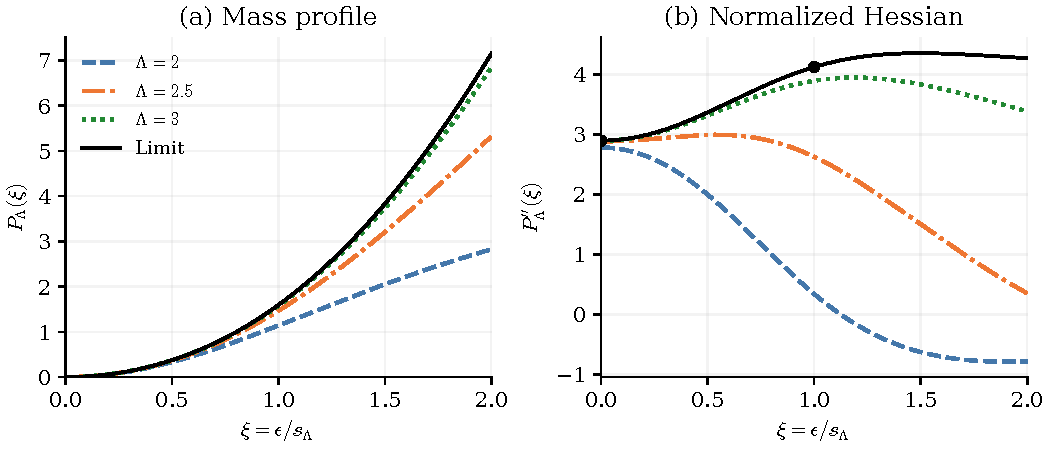
\includegraphics[width=\textwidth]{figures/output/mass-profile.pdf}
\caption{The exact normalized mass difference $P_\Lambda$ and normalized
Hessian $P_\Lambda''$, with their limits $P$ and $P''$.
The marked limiting Hessian values at $\xi=0,1$ differ by $\Delta$;
their original parameter separation tends to zero. The coordinate scale is
$s_\Lambda=\sqrt{2p}/\rho_\Lambda\sim\sqrt2\Lambda^2e^{-\Lambda^2/2}$.
The curves illustrate a proved static limit; they are not numerical
phase-flow trajectories.}\label{fig:profile}
\end{figure}
\FloatBarrier

\subsection{A negative ambient Levi direction}\label{subsec:levi}
For a phase angle $\theta\in(0,\pi)$, the real phase combination in
\cite[\S5.1]{hkkp26} is
$-\Rea\mathcal S_{\CC}+\cot\theta\,\Ima\mathcal S_{\CC}$.
On a complex gauge orbit the logarithmic determinant terms are locally
pluriharmonic. Its map-dependent candidate potential is therefore
\begin{equation}\label{eq:realpotential}
 \mathcal K_\theta(A,D)=\tr(CR(B))+c_\theta\tr\Ein(B),\qquad
 c_\theta=-\Rea z_0+\cot\theta\,\Ima z_0 .
\end{equation}
This formula is a construction from the explicit primitive; it is not
an assertion that \cite[\S5.4]{hkkp26} proves its ambient positivity.

\begin{proposition}\label{prop:negativelevi}
For $z_0=-1+\ii$, $z_1=1+\ii$ and $\theta=\pi/2$, the potential
\eqref{eq:realpotential} has a negative Levi direction on a complex
gauge orbit of the mixed family, for every $\Lambda>0$ and every
$\epsilon\in[0,1]$.
\end{proposition}

\begin{proof}
On one scalar acyclic summand put $a=|A|^2$, $b=|D|^2$.
The restriction of the potential is $aR(b)+c\Ein(b)$.
Its $A\overline A$ Levi entry is $R(b)>0$.
The Schur complement of that entry is
\begin{equation}\label{eq:levischur}
 e^{-b}[c-a\rho(b)],\qquad
 \rho(b)=\frac{b-1+e^{-b}}{b(1-e^{-b})}.
\end{equation}
Indeed the $D\overline D$ entry is
$a(R'+bR'')+ce^{-b}$, and the squared mixed entry divided by
$R$ is $ab(R')^2/R$; using $bR'=e^{-b}-R$ gives
\eqref{eq:levischur}.
For $b>0$, $\rho(b)>1/2$: the sign of $2\rho-1$ is the sign
of $b-2+(b+2)e^{-b}$, whose derivative is
$1-(b+1)e^{-b}>0$ and whose value at zero is zero.
Thus $c=1$, $a=4$ gives a negative direction for every $b>0$.

Realize this scalar restriction by taking $T_1=2\id$ and $T_2=T_3=0$
while keeping the balanced $B_j$ fixed. Vary one acyclic diagonal
entry of $D$ and the corresponding entry of $T_1$.
Independent nonzero complex rescalings of that acyclic source line
and its degree-one target line realize these two local variables
within one complex gauge orbit. Their potential is the scalar
expression above plus a constant, proving the assertion.
\end{proof}

An object-dependent additive constant cannot repair this negative
direction along the same metric orbit. The proposition obstructs a
generally plurisubharmonic ambient potential with the prescribed
phase primitive. It does not exclude a positive limiting cohomology
metric or every possible construction made directly on a quotient.

\subsection{Quantities and derivative domains}
For clarity, the static estimates concern the following distinct
objects, at fixed external $D=[0,F]$, $\sigma_{\min}(F)\geq\Lambda$,
and fixed reference metrics. The profile rows further specialize to
$F=\Lambda\id$ and the indicated family:

\begin{center}
\begin{adjustbox}{max width=\textwidth,center}
\begin{tabular}{lll}
\toprule
Quantity & Coordinate derivatives & Conclusion\\
\midrule
Coefficient $\Omega_F$ & bounded real $B,T$ coordinates
 & $C^k$ error $O_k(\Lambda^{-2})$\\
Relative primitive & the same coordinates
 & $C^k$ error $O_k(\Lambda^{-2})$\\
Trace-norm mass & the same coordinates
 & $C^0$ error $O(\Lambda^{-2})$, $C^1$ error $O(\Lambda^{-1})$\\
Mass in \eqref{eq:profilemixing} & surviving parameter $\epsilon$
 & $C^2$ convergence; $C^{2,\alpha}$ seminorms diverge\\
Normalized profile & $\xi=\epsilon/s_\Lambda$ on compact intervals
 & $C^k$ convergence for every fixed $k$\\
\bottomrule
\end{tabular}
\end{adjustbox}
\end{center}
No all-orders derivative conclusion for
$(\Omega_\Lambda\Omega_\Lambda^\dagger)^{1/2}$, the polar phase,
or an actual flow trajectory is contained in this table.

\section{The limiting quotient and a restricted positive construction}
\label{sec:geometry}

We first identify the limiting primitive under specified changes of
presentation. We then give a finite-scale positive construction with
additional hypotheses. Proposition~\ref{prop:negativelevi} rules out
extending its ambient positivity to all mixed presentations by the same
primitive.

\subsection{Relative primitives and elementary cancellations}
Fix Hermitian reference data on a surviving source $H$ and target $W$.
Let $C$ be an acyclic source sector and
$D=[0,F]:H\oplus C\to U$, where $F:C\to U$ is invertible.
Evaluate the primitive on metrics $h_V=h_H\oplus h_C$ and write
$A_j=[B_j,T_j]$. The metrics on $C,U$ and the map $F$ are fixed
throughout the static arrow-coordinate comparison.
Put $P_F=F^\dagger F$ and
$\lambda=\lambda_{\min}(P_F)>0$.
The zero-arrow acyclic primitive is
\begin{equation}\label{eq:acyclicprimitive}
 \mathcal S_{\ac}
 =z_0(\log\det h_C-\log\det h_U)+z_0\tr\Ein(P_F).
\end{equation}
With fixed determinant volume forms, subtracting this declared
expression from \eqref{eq:primitive} gives
\begin{equation}\label{eq:relativeprimitive}
 \begin{split}
 \mathcal S_{\mathrm{rel}}
 ={}&z_0\log\det h_H+z_1\log\det h_W-q_h(B)\\
 &-\sum_j\tr\bigl(T_jR(P_F)T_j^\dagger\bigr),\qquad
 q_h(B)=\sum_j\norm{B_j}_{\HS,h}^2 .
 \end{split}
\end{equation}
For fixed $F$ and acyclic metric data,
$0\leq R(P_F)\leq\lambda^{-1}\id$.
Thus the last term has absolute value at most
$\lambda^{-1}\sum_j\norm{T_j}_{\HS}^2$ and has
$O(\lambda^{-1})$ bounds for every fixed derivative in bounded
real $B,T$ coordinates. This is a relative static comparison, not
a constant subtraction on the full metric orbit.

Several elementary compatibilities follow from this exact formula.
For mutually orthogonal acyclic sectors with
$F=\diag_a(\Lambda_a\id)$, the error is
\begin{equation}\label{eq:sectorerror}
 -\sum_aR(\Lambda_a^2)\sum_j\norm{T_j^{(a)}}_{\HS}^2.
\end{equation}
The subtractions and removals of these sectors commute. Their bound
depends on $\min_a\Lambda_a$, not on the ratios of the scales.
This is an assertion for the displayed block decomposition, not
for interacting acyclic differentials without such a decomposition.

An elementary source shear
$g_V=\left(\begin{smallmatrix}\id&S\\0&\id\end{smallmatrix}\right)$,
where $S:C\to H$, leaves $D$ unchanged and replaces
$T_j$ by $T_j-B_jS$. The cohomology maps remain $B_j$.
For bounded data the two error terms in \eqref{eq:relativeprimitive}
both tend to zero, so their limits agree.
The same holds for every fixed derivative after composition with a
holomorphic parameter chart whose shear has bounded derivatives.
The two reference presentations must retain the same cohomology
Hermitian data, or transport them by a specified holomorphic isometry.
This does not assert equality at finite scale under a nonunitary shear
with unchanged ambient metrics.

Constant unitary frame changes preserve the comparison when they
transport $F$ and $T_j$ together. With unequal scales, a rotation of
acyclic frames generally changes the displayed matrix of $F$.
Rotating only the arrows while holding that matrix fixed is not the
claimed invariance.

Now specialize to $\dim H=\dim W=n>0$, $z_0=-1+\ii$, $z_1=1+\ii$.
The total cohomology charge is $2n\ii$, of phase $\pi/2$.
At fixed reference metrics, the limiting real arrow potential is
\begin{equation}\label{eq:limitpotential}
 K_H(B)=q(B)=\sum_j\norm{B_j}_{\HS}^2.
\end{equation}
Its Levi form is the usual positive flat form. The limiting
metric-direction function is
$q_h(B)+\log\det h_H-\log\det h_W$.
Its critical equations are
\begin{equation}\label{eq:ordinarybalance}
 \sum_jB_j^\dagger B_j=\id_H,\qquad
 \sum_jB_jB_j^\dagger=\id_W.
\end{equation}
The equality of dimensions is necessary by taking traces.
The resulting orbit-type K\"ahler quotients are the ordinary quiver
quotients. Their existence is classical; the calculation above
identifies the limiting potential and its normalization for these
presentations.

\subsection{An explicit finite-scale restriction}
Let $X=\operatorname{Hom}(H,W)^k$,
$G=\GL(H)\times\GL(W)$ and $K=\U(H)\times\U(W)$, acting by
$B_j\mapsto g_WB_jg_H^{-1}$. Take finitely many acyclic copies
$C_a=U_a=H$. Fix positive external scales $\Lambda_a$ and constant
matrices $L^{(a)}$ on the arrow-index space $\CC^k$ such that
\begin{equation}\label{eq:arrowmixing}
 (L^{(a)})^\dagger L^{(a)}=\kappa_a^2\id_k,\qquad \kappa_a\geq0.
\end{equation}
At least one $\kappa_a$ may be positive, so mixing need not vanish.
Define the holomorphic family of presentations
\begin{equation}\label{eq:graphfamily}
 T_j^{(a)}=\sum_lL_{jl}^{(a)}B_l,\qquad
 D=[0,\diag_a(\Lambda_a\id_H)].
\end{equation}
Its equivariance is for the embedding
\[
 g_V=\diag(g_H,g_H,\ldots,g_H),\qquad
 g_U=\diag(g_H,\ldots,g_H),\qquad g_W=g_W.
\]
It is not equivariant as a family with fixed graph data under the
entire presentation gauge group.

Transport $h_H$ to every $C_a$ and $U_a$, and retain $h_W$ on $W$.
All scales, arrow-index matrices and these fixed copy identifications
are held constant in the following tangent and metric comparisons.
Then $D^\dagger D$ on the $a$th copy is $\Lambda_a^2\id$ and
\[
 \sum_j\norm{T_j^{(a)}}_{\HS,h}^2
 =\kappa_a^2 q_h(B),\qquad
 \log\det h_V-\log\det h_U=\log\det h_H.
\]
Consequently the pullback of \eqref{eq:primitive}, after subtraction
of the constant $z_0n\sum_a\Ein(\Lambda_a^2)$, is exactly
\begin{equation}\label{eq:graphprimitive}
 \mathcal S_{\CC,\Lambda}
 =z_0\log\det h_H+z_1\log\det h_W-\alpha_\Lambda q_h(B),\qquad
 \alpha_\Lambda=1+\sum_a\kappa_a^2R(\Lambda_a^2)>0.
\end{equation}
This subtraction is constant on the specified tied-metric family,
as well as in $B$ at fixed scales. In contrast, it is not constant
on the full metric space of the complex.
The real arrow potential at phase $\pi/2$ is
$K_\Lambda=\alpha_\Lambda q$. Its metric and form are
$\alpha_\Lambda g_{\mathrm{flat}}$ and
$\alpha_\Lambda\omega_{\mathrm{flat}}$.
Their positivity follows directly from this formula.

\begin{proposition}\label{prop:quotientisometry}
For each fixed collection of data in
\eqref{eq:arrowmixing}--\eqref{eq:graphfamily}, the map
\begin{equation}\label{eq:scaling}
 \sigma_\Lambda:B\longmapsto\alpha_\Lambda^{-1/2}B
\end{equation}
induces an isometry on each connected smooth orbit-type stratum
from the ordinary balanced K\"ahler quotient to the quotient defined
by $K_\Lambda$ at the same central moment level.
It is the identity on the corresponding polystable cohomology
isomorphism classes.
The isometry preserves lengths, intrinsic distances and metric
completions on identically specified path domains.
\end{proposition}

\begin{proof}
Identify the Lie algebra dual with pairs of Hermitian matrices using
the fixed moment-map normalization
\[
 \mu_\alpha(B)=
 \left(-\alpha\sum_jB_j^\dagger B_j,\,
        \alpha\sum_jB_jB_j^\dagger\right),\qquad
 \eta=(-\id_H,\id_W).
\]
Let $Z=\mu_1^{-1}(\eta)$ and
$Z_\Lambda=\mu_{\alpha_\Lambda}^{-1}(\eta)$.
The diagonal scalar circle acts trivially; it may be retained as an
ineffective subgroup, and $\eta$ annihilates its Lie algebra since
the dimensions are equal. We do not assume freeness of the action.
These finite-dimensional holomorphic Hamiltonian reductions have
the usual smooth K\"ahler structures on connected orbit-type strata
\cite{sl91,sj95}. The quiver Kempf--Ness correspondence identifies
their points with polystable representations
\cite[\S6]{king94}. The hypotheses apply here: the ambient space is
flat K\"ahler, $K$ is compact, the level is central, and the source
Gram component controls $q(B)$, making the moment map proper.

The map $\sigma_\Lambda$ is a $K$-equivariant bijection from $Z$
to $Z_\Lambda$, preserving every stabilizer subgroup. It satisfies
\[
 \sigma_\Lambda^*(\alpha_\Lambda g_{\mathrm{flat}})
 =g_{\mathrm{flat}},\qquad
 \sigma_\Lambda^*(\alpha_\Lambda\omega_{\mathrm{flat}})
 =\omega_{\mathrm{flat}}.
\]
For clarity, if $v$ is a tangent lift and $\xi_X$ an infinitesimal
$K$-orbit vector, then
\[
 d\sigma_\Lambda(v)=\alpha_\Lambda^{-1/2}v,\qquad
 \xi_X(\sigma_\Lambda B)=\alpha_\Lambda^{-1/2}\xi_X(B).
\]
It follows directly that
\[
 \inf_{\xi\in\mathfrak k}
 \alpha_\Lambda\norm{d\sigma_\Lambda(v)+\xi_X(\sigma_\Lambda B)}^2
 =\inf_{\xi\in\mathfrak k}\norm{v+\xi_X(B)}^2.
\]
These are the squared reduced tangent norms. Stabilizer directions contribute
zero orbit vectors and cause no inverse estimate.
Furthermore $\sigma_\Lambda$ is the action of
$(\id_H,\alpha_\Lambda^{-1/2}\id_W)\in G$, so it leaves the
representation isomorphism class unchanged.

For the path statement, fix a $K$-invariant subset $\mathcal P\subset Z$
and use $\sigma_\Lambda(\mathcal P)$ on the other side.
Choose piecewise smooth paths within connected orbit-type strata,
with any allowed concatenations specified identically via
$\sigma_\Lambda$. The equality of tangent norms preserves every
admissible path length and hence their infimum on each finite-distance
component. If this convention first produces a pseudometric, divide
by zero distance on both sides. The resulting metric spaces, and
therefore their metric completions, are isometric.
No identification with a separate algebraic compactification is used.
\end{proof}

The finite-scale identity is elementary after \eqref{eq:graphprimitive};
it is not a general relative estimate for arbitrary mixing.
For the rank-two family \eqref{eq:balancedfamily}, scalar rescaling
preserves its stabilizer jump exactly, so this restricted quotient
identity remains valid without an orbit gap.

As a concrete example, take one copy and $L=\kappa\id_k$, $\kappa>0$.
Then $T_j=\kappa B_j$, and the off-diagonal block of the source
arrow Gram matrix is $E_H=\kappa C_H$.
It equals $\kappa\id$ on $Z$ and
$(\kappa/\alpha_\Lambda)\id$ on $Z_\Lambda$.
In either case it is nonzero, so the full source arrow Gram matrix
does not commute with $D^\dagger D=\diag(0,\Lambda^2\id)$.
This is mixing in the specified orthogonal Hermitian presentation.
The nonunitary shear $S=\kappa\id$ removes it algebraically, so
the example is not asserted to be an intrinsically nonsplit complex.

For a set $I$ of retained acyclic copies, put
$\alpha_I=1+\sum_{a\in I}\kappa_a^2R(\Lambda_a^2)$.
The calibrated map between the $I$ and $J$ levels is multiplication
by $\sqrt{\alpha_I/\alpha_J}$. These factors telescope under
successive removals, proving order independence for this construction.
Constant unitary changes of frames transport the differential and
arrows together as above.

\subsection{Limits of the comparison}
The comparison fixes each $\Lambda_a$ and each $L^{(a)}$.
Varying $\Lambda_a$ in a tangent direction differentiates
$\alpha_\Lambda^{-1/2}$ and introduces an additional term;
Proposition~\ref{prop:quotientisometry} makes no metric assertion in
such total-parameter directions.
It also does not claim that the full phase flow preserves the
tied-metric family. Indeed that family keeps the norm of $D$ fixed,
whereas the cancellation theorems prove its growth.

Theorem~\ref{thm:intromixed} applies to ordinarily balanced initial
tuples $B\in Z$ with any finite positive number $\ell$ of these acyclic
copies. Indeed the combined acyclic rank is $r=\ell n$, and
\[
 \sum_{a,j}\norm{T_j^{(a)}}_{\HS}^2
   =n\sum_a\kappa_a^2=:M^2,\qquad
 \sigma_{\min}(F_0)=\min_a\Lambda_a.
\]
If $\min_a\Lambda_a\geq\Lambda_*(n,M)$, the actual phase flow has
the theorem's cancellation and relaxation properties, independently
of the ratios of the initial scales. This applies for arbitrary $k$
and every stabilizer of the ordinarily balanced tuple.
The evolving metrics are those of the full phase flow, not metrics
constrained to remain in the family used for the quotient isometry.
The rescaled representative $\alpha_\Lambda^{-1/2}B$ is generally
not ordinarily balanced at the reference metrics, so the dynamical
theorem does not automatically apply to that representative.

Thus the general result of this section is the relative static
primitive limit under the declared elementary changes.
The finite positive metric is a restricted construction.
Neither result asserts a general metric on the moduli of all
complexes or an isometry under arbitrary derived equivalences.

\section{Further questions}\label{sec:questions}

The mass counterexample and the cancellation theorems concern the same
positive phase equation. They show that acyclic cancellation need not
come from trace-norm mass dissipation. For an invertible differential,
the contracting quotient $A_jD^{-1}$ supplies the missing control from
every initial metric. With a surviving source, estimates using only the
nonsingular cohomology block close the argument at large initial acyclic
scale. They allow arbitrary surviving tuples, unequal dimensions and
fixed upper-half-plane charges, uniformly in arrow count, stabilizers
and acyclic condition numbers.

Cancellation and relaxation have different hypotheses. For equal surviving
dimensions and charges $-1+\ii$, $1+\ii$, a finite infimum of the
cohomology Kempf--Ness function gives relaxation from nonbalanced initial
metrics. Its quantitative energy bound retains the initial excess
$\mathcal K(0)-\inf\mathcal K$. An arrow-norm bound alone need not bound
this excess: for a scalar one-arrow representation $B=b\ne0$ at standard
metrics, it is $|b|^2-1-\log|b|^2$, which diverges as $b\to0$.
Lower boundedness, and not attainment, is the analytic hypothesis used
in the proof. For arbitrary surviving representations that hypothesis
can fail even though large-scale cancellation still holds.

Removing the large-initial-scale assumption remains open for the mixed
theorem. The inequality
$s'\leq(-a+4\pi q/(b_0\lambda))s$ requires control of $q/\lambda$
before it becomes contractive; monotonicity of $\lambda$ alone supplies
no such bound. It is also natural to ask whether the mechanism extends
to longer complexes while retaining independence from positive
surviving orbit eigenvalues.

The integrated moment-map estimate gives no uniform final relaxation
rate, normalized surviving-metric limit, or parameter derivatives of
actual trajectories. These questions require additional control of the
surviving dynamics. The static results allow arbitrary fixed invertible
acyclic differentials but do not differentiate that differential.
For the explicit scalar-scale family, mass converges in $C^2$ and every
positive H\"older seminorm of its Hessian diverges. Optimal general
second-derivative estimates on the full arrow-coordinate space remain open.

The explicit primitive separates metric-direction exactness from
transverse positivity. Its negative ambient Levi direction excludes
one direct positive-potential construction. The limiting cohomology
metric and restricted finite-scale example leave open a general
quotient-only construction with its own normalization and compatibility
laws. Extensions to bundle complexes and singular geometric limits
require additional elliptic analysis; none follows from these
finite-dimensional results.

\begin{thebibliography}{HKKP26}

\bibitem[BL95]{bl95}
J.-M.~Bismut and J.~Lott,
\textit{Flat vector bundles, direct images and higher real analytic torsion},
J. Amer. Math. Soc. \textbf{8} (1995), no.~2, 291--363.
\href{https://doi.org/10.1090/S0894-0347-1995-1303026-5}{doi:10.1090/S0894-0347-1995-1303026-5}.

\bibitem[HKKP23]{hkkp20}
F.~Haiden, L.~Katzarkov, M.~Kontsevich and P.~Pandit,
\textit{Semistability, modular lattices, and iterated logarithms},
J. Differential Geom. \textbf{123} (2023), no.~1, 21--66.
\href{https://doi.org/10.4310/jdg/1679503804}{doi:10.4310/jdg/1679503804};
\href{https://arxiv.org/abs/1706.01073v2}{arXiv:1706.01073v2}.

\bibitem[HKKP26]{hkkp26}
F.~Haiden, L.~Katzarkov, M.~Kontsevich and P.~Pandit,
\textit{Towards categorical K\"ahler geometry},
preprint (2026), \href{https://arxiv.org/abs/2609.00978v1}{arXiv:2609.00978v1}.

\bibitem[High86]{higham86}
N.~J.~Higham,
\textit{Computing the polar decomposition---with applications},
SIAM J. Sci. Statist. Comput. \textbf{7} (1986), no.~4, 1160--1174.
\href{https://doi.org/10.1137/0907079}{doi:10.1137/0907079}.

\bibitem[King94]{king94}
A.~D.~King,
\textit{Moduli of representations of finite dimensional algebras},
Quart. J. Math. Oxford Ser. (2) \textbf{45} (1994), no.~4, 515--530.
\href{https://doi.org/10.1093/qmath/45.4.515}{doi:10.1093/qmath/45.4.515}.

\bibitem[Lew95]{lewis95}
A.~S.~Lewis,
\textit{The convex analysis of unitarily invariant matrix functions},
J. Convex Anal. \textbf{2} (1995), no.~1--2, 173--183.
\href{https://doi.org/10.68381/jca02012}{doi:10.68381/jca02012}.

\bibitem[Li95]{li95}
R.-C.~Li,
\textit{New perturbation bounds for the unitary polar factor},
SIAM J. Matrix Anal. Appl. \textbf{16} (1995), no.~1, 327--332.
\href{https://doi.org/10.1137/S0895479893256359}{doi:10.1137/S0895479893256359}.

\bibitem[PV09]{pv09}
P.-\'E.~Paradan and M.~Vergne,
\textit{Quillen's relative Chern character},
in \textit{Algebraic Analysis and Around},
Adv. Stud. Pure Math. \textbf{54}, Math. Soc. Japan, Tokyo, 2009,
255--291.
\href{https://doi.org/10.2969/aspm/05410255}{doi:10.2969/aspm/05410255};
\href{https://arxiv.org/abs/math/0702575v3}{arXiv:math/0702575v3}.

\bibitem[Sj95]{sj95}
R.~Sjamaar,
\textit{Holomorphic slices, symplectic reduction and multiplicities of
representations},
Ann. of Math. (2) \textbf{141} (1995), no.~1, 87--129.
\href{https://doi.org/10.2307/2118628}{doi:10.2307/2118628}.

\bibitem[SL91]{sl91}
R.~Sjamaar and E.~Lerman,
\textit{Stratified symplectic spaces and reduction},
Ann. of Math. (2) \textbf{134} (1991), no.~2, 375--422.
\href{https://doi.org/10.2307/2944350}{doi:10.2307/2944350}.

\end{thebibliography}

\end{document}
